% Bsp. eines Hauptteils

\begin{spacing}{1.2}

\chapter{Grundlagen}
\label{sec:grundl}

\section{Funktionsprinzip, Vorteile und Herausforderungen des modernen Cloud Computings}

\subsection{Definition und Funktionsweise}

Das National Institute of Standards and Technology (NIST) der Vereinigten
Staaten von Amerika definiert Cloud Computing im Abstract der NIST SP-800-145
folgendermaßen:\\

Cloud computing is a model for enabling ubiquitous, convenient, on-demand network access to a shared
pool of configurable computing resources (e.g., networks, servers, storage, applications, and services) that
can be rapidly provisioned and released with minimal management effort or service provider interaction.
This cloud model is composed of five essential characteristics, three service models, and four deployment
models.\\

Cloud Computing beschreibt ein Modell das es ermöglicht ortsunabhängig, zweckdienlich und
zeitunabhängig auf einen konfigurierbaren Pool an Computerresourcen (Netzwerke, Server,
Datenspeicher, Anwendungen und Services) zuzugreifen die schnell und mit minimalem
Aufwand und minimaler notwendiger Interaktion bereitgestellt und wieder abgebaut
werden können.
Dieses Cloud Modell beschreibt fünf essentielle Charakteristiken, drei Servicemodelle
und vier Bereitstellungsmodelle.\\

Weiter definiert das Dokument die fünf Charakteristiken in den folgenden Punkten:\\

\textbf{On-demand-self-service:} Der Nutzer kann eigenmächtig die benötigten Resourcen
automatisch bereitstellen, es wird keine menschliche Interaktion benötigt.

\textbf{Broad network access:} Auf Leistungen wird über das normale Internet mit standard
Mechanismen die die Nutzung von Thin Clients und Fat Clients (Smartphones, Tablets,
Laptops oder Workstations) fördern zugegriffen.
 
\textbf{Resource Pooling:}: Die Computerresourcen des Anbieters werden in einem gemeinsamen Pool
für mehrere Kunden in einem mandantentauglichen Modell bereitgestellt, physische und
virtuelle Resourcen werden nach dynamisch zugewiesen und entsprechend der Nachfrage
neu verteilt. Es wird eine empfundene Ortsunabhängigkeit hergestellt indem der Nutzer
kein genaues Wissen darüber besitzt wo sich dessen Resources befinden, auf höherem
Level wie beispielsweise dem Staat, der Region oder auch Rechenzentrum kann
der Ort vom Nutzer spezifiziert werden. Die bereitgestellten Resourcen beinhalten
zum Beispiel Datenspeicher, Rechenleistung, Rechenspeicher und Netzwerkbandbreite.

\textbf{Rapid Elasticity:} Rechenkapazitäten werden dehnbar bereitgestellt und abgebaut,
teilweise automatisch, um entsprechend der Nachfrage schnell hoch- und wieder
zurück skalieren zu können, Rechenkapazitäten erscheinen dadurch unbegrenzt und
zu jeder Zeit in jedem Umfang bereitgestellt werden.

\textbf{Measured Service:} Cloud systeme kontrollieren und optimieren Resourcennutzung
automatisch mithilfe eines Messungs-systems dass auf einer abstrakten Ebene den
entsprechenden Service (Datenspeicher, Rechenleistung, Benutzerkonten) überwacht,
kontrolliert und Bericht erstattet um sowohl für Anbieter als auch Kunden Transparenz
herzustellen.\\

Es wird zwischen drei grundlegende Cloud Service Modellen unterschieden: Infrastructure
as a Service (IaaS), Platform as a Service (PaaS) und Software as a Service (SaaS).

\begin{figure}[H]
  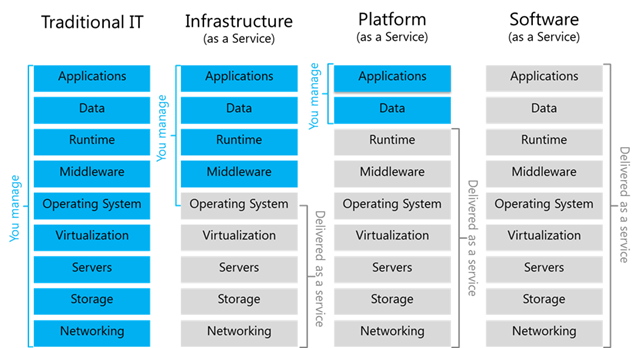
\includegraphics[width=1.0\textwidth]{fig/hauptteil/Service-Models.png}
  \caption{Die grundlegenden Cloud Service Modelle im Überblick}
  \centering
\end{figure}

\textbf{Infrastructure as a Service:} Der Nutzer hat die Fähigkeit Rechenleistung, Datenspeicher
Netzwerke und weitere fundamentale Computerresourcen bereitzustellen und beliebige Software
darauf zu betreiben, dazu können Betriebssysteme und Anwendungen gehören. Die
darunterliegende Infrastruktur wird vom Anbieter betrieben, der Nutzer  kann aber
eingeschränkte Kontrolle über bestimmte Komponenten haben, dazu gehören beispielsweise
Firewalls.

\textbf{Platform as a Service:} Der Nutzer verfügt über die Fähigkeit seine eingkaufte oder
selbst erstellten Anwendungen auf der Cloud Infrastruktur zu betreiben, die notwendige
Umgebung die über Sprachen, Bibliotheken, Tools und Services verfügt wird vom Anbieter
bereitgestellt. Die darunter liegende Infrastruktur mit Netzwerken, Servern,
Betriebssystemen und Speicher wird vom Anbieter betrieben, der Nutzer hat die Kontrolle
über die Anwendung und Konfiguration der Umgebung in der die Anwendung betrieben wird.

\textbf{Software as a Service:} Dem Nutzer wird der Zugriff auf die vom Anbieter in der
Cloud Infrastruktur betriebenen Softwareanwendung gewährt. Auf diese wird mithilfe
eines Thin oder Fat Clients zugegriffen, dabei kümmert sich der Nutzer nicht um den
Betrieb und die Konfiguration der darunterliegenden Cloud Infrastruktur wie
Netzwerke, Server, Betriebssystem, Speicher und die Anwendung selbst mit Ausnahme
eingeschränkter Nutzereinstellungen.

Die von NIST unterschiedenen grundlegenden Service Modellen können noch weiter
differenziert werden.
Ein Beispiel hierfür ist das Modell Function as a Service (FaaS) als Subset von PaaS.
FaaS erlaubt es Programmcode auszuführen ohne sich um die Bereitstellung weiterer 
Infrastruktur kümmern zu müssen wie es der Betrieb eines gewöhnlichen Microservices
verlangt.\\

In Art der Bereitstellung eines Cloud Services werden vier grundlegende Modelle
unterschieden; Public, Private, Hybrid und Community Cloud Modelle.\\

\textbf{Private Cloud:} Die Cloud Infrastruktur wird ausschließlich für die Nutzung durch eine einzige
Organisation mit mehreren Nutzern bereitgestellt. Besitz und Betrieb liegen dabei
entweder bei der selben Organisation, einer Drittpartei oder einer Kombination beider, 
die Infrastruktur kann dabei On- oder Off Premise betrieben werden.

\textbf{Public Cloud:} Die Public Cloud steht für die Nutzung durch die allgemeine Öffentlichkeit bereit.
Die Cloud Infrastruktur befindet sich im Besitz eines Unternehmens, Bildungseinrichtung,
Regierungsorganisation oder einer Kombination aus diesen und wird auch von der selben
Organisation On Premise betrieben. 

\textbf{Community Cloud:} Eine Community Cloud wird von einer Gemeinschaft von Nutzern mit gemeinsamen
Anliegen eingesetzt. Der Besitz und Betrieb liegen dabei bei einem oder mehreren
Mitgliedern dieser Gemeinschaft, einer Drittpartei und kann Off oder On Premise betrieben
werden.

\textbf{Hybrid Cloud:} Die Hybrid Cloud besteht aus einer Kombination der beschriebenen Modelle
(Public, Private und Community). Diese bilden dabei eigene Instanzen die aber durch
standardisierte oder proprietäre Schnittstellen den Transfer von Daten und Anwendungen
zwischen den Instanzen erlauben.

\subsection{Zu erwägende Vor- und Nachteile des Einsatzes von Cloud Computing}

\subsubsection{\textbf{Vorteile und Treiber der Adoption von Cloud Computing}}

\textbf{Wirtschaftliche Vorteile:} Ein Vorteil in der Nutzung von Cloud Computing
kann darin liegen dass ein Großteil der für den Betrieb notwendigen Infrastruktur
nicht mehr vom Unternehmen selbst eingakuft, eingerichtet und betrieben werden
muss (vgl. linke Seite Abb 2.1). Potentiell hohe Kosten die bereits vor der
Inbetriebnahme eines Systems mit einem höheren Risiko aufgewendet werden mussten
stellen in Form von individuell geringeren laufenden Beträgen ein deutlich
reduziertes Risiko da.\\
Sofern der Einsatz von Cloud Computing in einer sinnvollen und korrekten
Weise erfolgt können je nach Fall die Gesamtkosten um einen hohen Anteil reduziert
werden.\\
Die Gesamtkostenersparnisse stehen auch im Zusammenhang mit Skaleneffekten die für
große Cloudanbieter gelten. Der Betrieb eines einzelnen Servers ist im Verhältnis
mit bedeutend höheren Kosten verbunden als das hinzufügen eines äquivalenten
System zu einem Rechenzentrum im Betrieb von AWS oder einem vergleichbaren
Anbieter.

\textbf{Skalierbarkeit:} Besonders für schnell wachsende Unternehmen ist die
Option der schnellen Skalierbarkeit einer der prominentesten Vorteile der Cloud.
Es kann nicht nur auf vorhersagbare Anstiege (zum Beispiel ausgelöst durch
eine Verkaufsaktion) sondern auch auf unvorhersehbare Ereignisse reagiert werden.
Zusätzlich ist es möglich diese Skalierung nicht nur bis zu einem bestimmten Limit,
sondern nahezu unendlich zu betreiben. Wichtig ist auch dass sowohl auf steigende
als auch sinkende Nachfrage reagiert werden kann.

\textbf{Resilienz:} In einem worst case Szenario kann ein ganzes Rechenzentrum
durch unvorhergesehen Ereignisse wie beispielsweise Brände, Naturkatastrophen
oder anderes vollständig zerstört werden. Selbst wenn Backup-Rechenzentren
verfügbar sind ist eine übertragung der Operationen kein trivialer Ablauf und
birgt oft nicht außer Acht zu lassende Risiken. Die Flexibilität der Cloud
erlaubt es die gesamte Infrastruktur mit sehr geringem Aufwand in nicht
betroffene Regionen zu verlagern und die Kontinuität der Geschäftstätigkeiten
mit minimaler Unterbrechung aufrecht zu erhalten.

\textbf{Security:} Security Aspekte können sowohl einen Vor- als auch Nachteil
von Cloud Computings darstellen. Hier sollen zuerst Vorteile dargelegt werden,
potentielle Probleme werden im nächsten Unterkapitel beschrieben.
Die technischen Möglichkeiten und besonders auch die Wahrnung des Themas
Sicherheit in der Cloud unterlagen und unterliegen auch immernoch einem
deutlichen Wandel. Cloud Anbieter investieren
viele Resourcesn in Sicherheit und stellen dem Nutzer zum Beispiel bereits sicher
implementierte Verschlüsselungen zur Verfügung oder bieten einen gewissen
Schutzen vor Denial-of-Service Angriffen durch die natürliche Skalierbarkeit.\\

\subsubsection{\textbf{Nachteile und Risiken}}

\textbf{Netzwerkabhängigeit:} Da der Zugriff auf Cloud Dienste über das
Internet erfolgt entsteht dadurch entsprechend auch eine hohe Abhängigkeit.
Eine stabiele und schnelle Netzwerkanbindung ist vorraussetzung dass effektiv
gearbeitet werden kann, bei lokal gehosteten Systemen ist diese Abhängigkeit
entsprechend geringer.

\textbf{Vendor Lock-in:} Bei der Nutzung eines Cloud Anbieters entsteht die
Gefahr sich zu sehr in Abhängigkeit eines einzelenen Anbieters zu begeben.
Im Fall einer Änderung der Nutzungsbedingungen oder einer Änderung im
Bezahlmodell die den eignen Interessen stark entgegen steht besteht die Gefahr
bereits so abhängig von diesem Anbieter zu sein dass die Kosten eines Wechsels
derart hoch ausfallen dass man gezwungen ist die Bedingugen zu akzeptieren.

\textbf{Security und Privacy:} Sicherheitsrisiken sind einer der meistgenannten
Gründe die gegen Cloud Computing sprechen, besonders im Fall der Nutzung einer
Public Cloud. Die Gefahr dass Daten in die Hände dritter gelangen kann zum
zum Beispiel nicht vollständig ausgeschlossen werden. Da die Verantwortung über
die Sicherheit der Daten dem Cloud Anbieter unterliegt kann es auch zu Problemen
in Hinsicht der Privateheit der Daten kommen, sollte eine Regierungsorganisation
Zugriff auf bestimmte Daten eines Nutzer verlangen könnten diese ohne dessen
Einverständnis gewährt werden.

\textbf{Kosten:} Auch wenn die Nutzung von Cloud Computing mit dem Vorteil
geringerer Kosten beworben ist dies nicht zwingend garantiert. Werden die
vorhandenen Systeme ungünstig verwendet, zum Beispiel bleiben viele gebuchte
Ressourcen ungenutzt und IP-Adressen unverwendet, können hohe Kosten entstehen,
auch in der Phase des Übergangs zu Cloud Computing können höhere Kosten
entstehen als in einem vergleichbaren Zeitraum davor.


\subsection{\textbf{Grundlegende Erklärung von DevOps}}

Die exakte Definition und Abgrenzung des Begriffes DevOps ist ein Thema über
das es keine uniform akzeptierte allein gültige Definition und Abgrenzung gibt.
Im allgemeinen aber bezeichnet DevOps eine stärkere Vereinigung der Entwicklungs-
(Dev) und Betriebs- (Ops) Teams eines Softwareprojekts durch die Anwendung
einer effektiveren Arbeitskultur und -philosophie mit neuen Methoden, Werkzeugen und
Prozessen. Verschiedene Organisationen legen hierbei in ihrer Definition die
Schwerpunkte auf unterschiedliche Aspekte.
Als Beispiel betont Amazon hierbei besonders die schnelle Auslieferung neuer
Produkte ("ability to deliver applications and service at high velocity"),
Microsoft
die Kollaboration zwischen den beteiligten Teams ("DevOps enables formerly
siloed roles - development, IT operations, quality engineering, and security -
to coordinate and collaborate to produce better, more reliable products.").\\
Das DevOps Reasearch and Assessment (DORA) Team
hat über sieben Jahre mit 32.000 Beteiligten die Praktiken und 
Fähigkeiten untersucht die hohe Leistungsfähigkeit bei Entwicklung und
Auslieferung von Sofware fördern. Eine Übersicht über die Erkenntnisse dieser
Studie ist als Diagramm im Anhang ... zu finden.\\
Infrastructure as Code spielt als Werkzeug für die automatisierte Bereitstellung
der benötigten Computerresourcen eine wichtige Rolle im DevOps Prozess.

\subsubsection{\textbf{GitOps als Werkzeug für Continuous Delivery im Rahmen von DevOps}}

GitOps wird von Gitlab als ein betriebliches Rahmenkonzept (operational
Framework) defniert das DevOps Best Practices in der automatiserten
Bereitstellung von Infrastruktur anwendet.
GitOps benötigt dabei drei Hauptkomponenten:\\
Infrastructure as Code, Merge Requests und CI/CD.
Organisationen die mit einer ausgereiften Anwendung der DevOps Kultur arbeiten
können über GitOps hunderte Male pro Tag neuen Code auf den Produktionsservern
installieren. Im praktischen Teil dieser Arbeit wird GitOps verwendet um
da es eine einfache Integration mit Github ermöglicht, Github selbst
wird als Versionskontrollsystem verwendet da es weithin etabliert und breit
unterstützt ist und von der Novatec Consulting GmbH bevorzugt eingesetzt wird.

\subsection{Überblick über die wichtigsten Public Cloud Service Provider}
Da der Kern der Arbeit die Infrastructure as Code Unterstützung der
wichtigsten Cloud Service Provider in deren Public Cloud untersucht soll hier
ein kurzer Überblick über den aktuellen Markt in diesem Bereich gegeben werden.

\begin{figure}[H]
  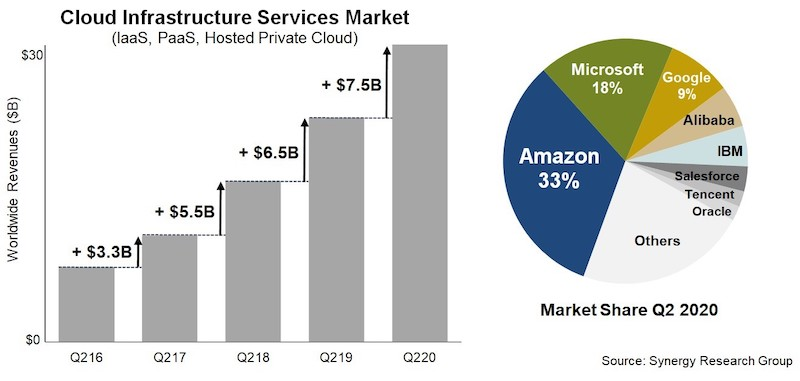
\includegraphics[width=1.0\textwidth]{fig/hauptteil/CIS_Q220.jpg}
  \caption{CSP Market Share Q2 2020 nach Umsatz}
  \centering
\end{figure}

\textbf{1. Amazon: } Amazon besitzt mit 33\% den größten Anteil am Markt.
Die Amazon Elastic Compute Cloud (EC2) ist die älteste der aktuell großen Cloud
Computing Plattformen, der erste Release fand im August 2006 statt.

\textbf{2. Microsoft: } Microsoft stellt den zweitgrößten Anteil am Markt mit
18\%, der erste Release von Microsoft Cloud Computing Service Microsoft Azure
erfolgte im Oktober 2008. Gemeinsam besaßen Amazon und Microsoft 2020 über 50\%
des gesamten Marktes.

\textbf{3. Google: } Google's Google Cloud Platform steht mit 9\% an dritter
Stelle. Google Compute Engine, die IaaS Komponente der Cloud Services von
Google wurde im Juni 2012 veröffentlicht.

\textbf{4. Alibaba Cloud: } Die viertgrößte Cloud Plattform ist die
Alibaba Cloud der Alibaba Group. Alibaba Cloud bietet zusätzlichzu seinem
Elastic Compute Service (ECS) einen dedizierte GPU basierten Service an. 

\textbf{5. IBM Cloud: } Die aktuell fünftgrößte Cloud Computing Plattform ist
die IBM Cloud von IBM. Bis Juni 2013 eine eigene Firma unter dem Namen Softlayer
wurde diese von IBM übernommen und 2017 gemeinsam mit den anderen Cloud Services
der Firma in ein einheitliches Portfolio unter dem Namen IBM Coud aufgenommen.\\

\begin{figure}[H]
  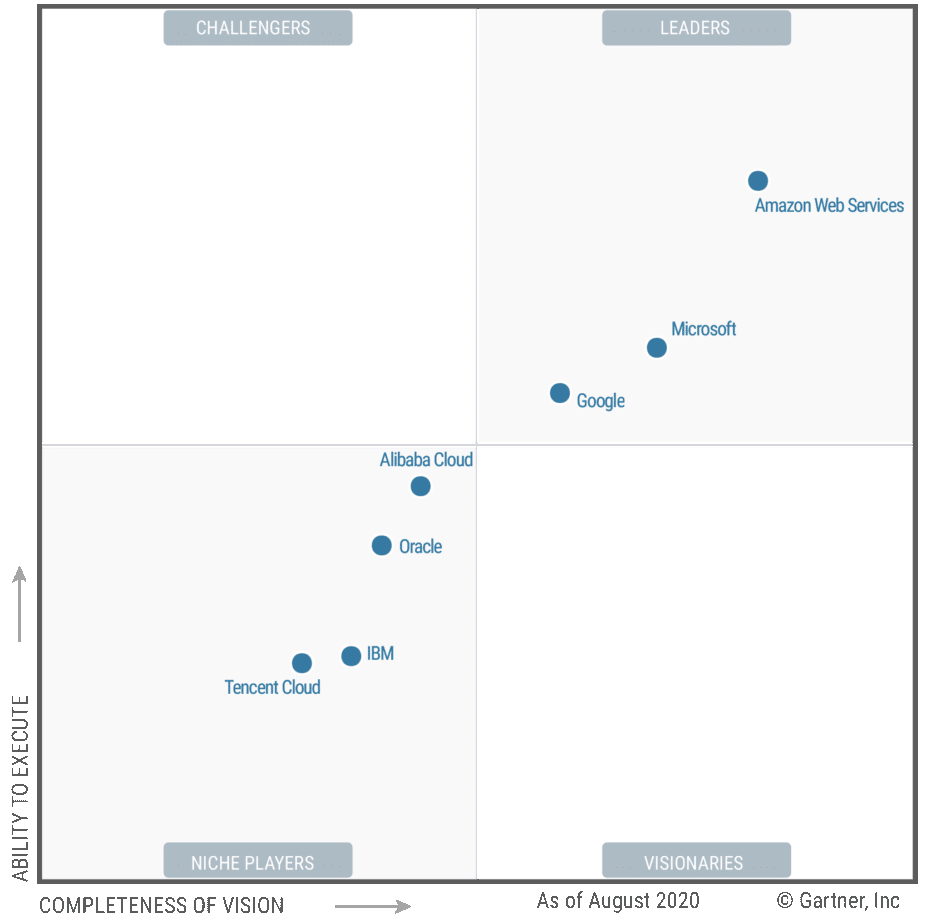
\includegraphics[width=1.0\textwidth]{fig/hauptteil/Gartner-Magic-Quadrant.png}
  \caption{CSP Gartner Magic Quadrant August 2020}
  \centering
\end{figure}

Der Gartner Magic Quadrant für Cloud Service Provider bietet einen groben
Überblick über den Umfang der Angebote (Completeness of Vision) und
die Ausgereiftheit einer Plattform (Ability to Execute). Deutlich erkennbar
ist hier die Vormachtsstellung von Amazon gegenüber Microsoft und Google sowie
der Abstand von Google zum nächst größten Anbieter Alibaba Cloud.
TODO: Irgendwas mit IBM Ability to Execute vs Marktanteil verglichen mit Oracle


\section{Infrastructure as Code}

Infrastructure as Code beschreibt einen Ansatz zur Automatiesierung der
Bereitstellung von Infrastruktur basierend auf Methoden aus der
Softwareentwicklung (vgl Kief Morris Infrastructure as Code S.4).\\
Statt eines manuellen Aufbaus und direkter Konfiguration der einzelnen
Komponenten werden maschinenlesbare Dateien verfasst welche dann von einem
IaC Tool eingelesen und verarbeitet werden. Dabei kommen bevorzugt
deklarative Sprachen zum Einsatz deren höhere Abstraktion mehr Flexibilität
als ein imperativer Ansatz erlaubt.
(vgl. https://docs.microsoft.com/en-us/devops/deliver/what-is-infrastructure-as-code)

\subsection{Technologischer Wandel und das Cloud Age Mindset}

Durch die Technologien der Cloud ist es möglich eine gewünschte
IT-Infrastruktur sehr viel schneller bereitzustellen als
zuvor möglich. Statt des Einkaufs, Anschließens und Einrichtens eines
physischen Servers das, je nach Szenario einen Zeitraum von mindestens
mehreren Stunden oder Tagen bis zu Wochen gedauert hätte können
virtuelle Resourcen in der Cloud in wenigen Minuten bereitgestellt werden.
Der schnellere Ablauf wird durch die Automatisierung von Prozessen wie etwa
der Bereitstellung der Infrastruktur mithilfe von IaC Tools noch verstärkt,
nicht nur bei der initialen 
Mit diesen Veränderungen wird das Management und die Erweiterung der
bestehenden Systeme jedoch nicht unbedingt einfacher (vgl IaC Kief Morris S.3),
die Verwendung der alten IT-Governance Modelle (TODO Fußnotenerklärung) die
sich bisher bewährt haben sind jedoch aufgrund der Veränderungen ungeeignet.
Kief Morris stellt die fundamentalen Unterschiede des Arbeitens mit
Cloud-Technologien mithilfe der folgenden Tabelle dar.

\begin{figure}[H]
  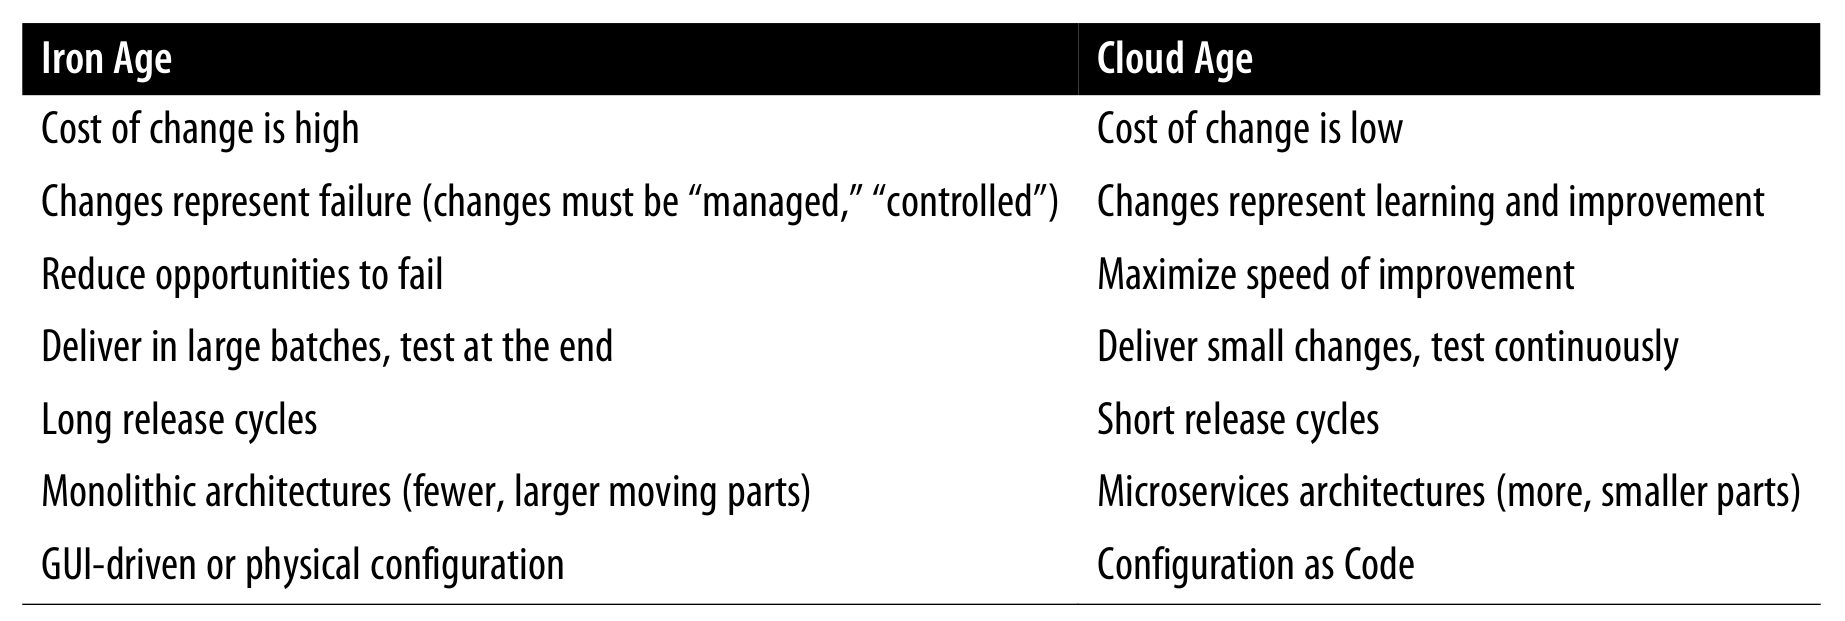
\includegraphics[width=1.0\textwidth]{fig/hauptteil/Tabelle_1-2_IaC.png}
  \caption{Iron Age vs Cloud Age}
  \centering
\end{figure}

Veränderungen in der 'Iron Age' sind aufwändig und teuer und stellen ein
Risiko dar, es wird versucht diese Risikopunkte zu reduzieren daher werden
viele Veränderung gebüdelt getestet und eingeführt wodurch lange
Release-Zyklen entstehen. Die Architekturen die dadurch befördert werden
sind eher monolytisch die Konfiguration erfolgt eher mithilfe von GUI
gesteuerten Programmen oder physischen, zum Beispiel wenn ein neuer Server
in ein Netzwerk eingebunden wird. Veränderungen in der Cloud stellen
fast genau das Gegenteil dar, daher wird erkennbar dass eine auf die
'Iron Age' zugeschnittene Arbeitsweise für die Cloud nicht effektiv ist,
es ist ein neues Cloud Age Mindset das die rechte Spalte der Tabelle
verinnerlicht erforderlich um die Vorteile der Cloud
wirklich effektiv nutzen zu können.

\subsection{Vorteile von IaC und durch IaC gelöste Probleme des
manuellen Provisionings}

\textbf{Kein Configuration Drift durch einheitliche Codebase:}
Configuration drift bezeichnet eine über die Zeit
wachsende Abweichung zweier ursprünglich identischer Systeme. Wird ein
gleiches System, zum Beispiel ein Applikationsserver, in verschiedenen
Umgebungen eingesetzt stellen diese oftmals auch leicht verschiedene
Anforderungen auf die dann mit Optimierungen, etwa in Form spezifischer
Konfigurationsdetails, reagiert werden kann. Wird nun das ursprüngliche
System geupdated werden individuelle, oft undokumentierte Anpassungen
nicht berücksichtigt und ein Update kann unbequeme Konsequenze nach
sich ziehen. Werden alle Veränderungen in einer einheitlichen
Codebase verwaltet und Updates häufig vorgenommen verhindert man
starken Configuration Drift der über Zeit stattfindet

\textbf{Wiederverwendbarkeit durch einheitlichen Code:}
Ein weiterer Vorteil der durch die Verwendung einer einheitlichen
Codebase entsteht ist die Wiederverwendbarkeit und Repoduzierbarkeit
eines Systems. Wenn ein identisches System an einer anderen Stelle
aufgebaut werden soll oder sollte das System aus unvorhergesehen
Gründen in seiner Gesamtheit verloren gehen kann es schnell und mit
verhältnismäßig geringem Aufwand reproduziert werden.
Ein dazu passender Ausdruck in Bezug auf Server ist 'Cattle not Pets'.
Statt sich individuell und mit großem Aufwand um einzelne Server zu
kümmern wie man es etwa mit dem eigenen Haustier tut sollten Server
wie leicht ersetzbares Vieh behandelt werden.

\textbf{Schnelleres Provisioning durch Cloud:} Ein bereits häufig
angesprochener Vorteil ist die schnelle Bereitstellung, auf tiefere
Erklärung kann daher hier verzichtet werden.

\textbf{Schnellerer Profit:} Schnellere Bereitstellung der Hardware
und schnellere Auslieferung von Software die durch DevOps Methoden
begünstigt werden erzeugen entsprechend auch schneller einen Mehrwert.

\textbf{Einheitliches Tooling in Dev, Ops und weiteren Beteiligten Teams:}
Verwendung von IaC
fördert die einheitlicheres Tooling in allen Bereichen die mit einem
Softwareprodukt in Zusammenhang stehen. Cloud Technologien fördern und
ermöglichen diese Vereinheitlichung, manuelles Provisioning ohne ein
Cloud Modell erschwert dies oder macht es sogar unmöglich.

\textbf{Stärkere Automatisierung im Arbeitsablauf:} Automatisierung
bedeutet immer einen gewissen upfront Overhead, jedoch kann auf
längere Sicht deutlich von automatisierten Abläufen profitiert weren.
Ein Beispiel hierfür sind automatisierte und in eine CI/CD Pipeline
integrierte Tests.

\textbf{Höhere Zuverlässigkeit und Sicherheit durch schnelle Updates:}
Von eine Struktur die schnelle und häufige Veränderungen fördert
kann auch die Sicherheit und Zuverlässigkeit eines Systems profitieren.
Auf Sicherheitsrisiken kann in kurzer Zeit und ohne viel Aufwand
reagiert werden, eine unsichere Funktion kann etwa schnell durch
eine sichere Variante ausgetauscht werden, mögliche damit verbundene
Probleme können dann in automatisierten Tests erkannt werden wodurch
das System zuverlässig bleibt.

\textbf{Schnellere Fehlersuche und -behebung:}

Fehler die dennoch auftreten können dann durch den Einsatz kleinerer
Komponenten schneller isoliert, gefunden und behoben werden.
Monolithische Systeme erschweren dies durch dadurch dass weniger klar
isolierte Komponenten vorhanden sind die häufig mehr Abhängigkeiten
aufweisen und daher schwerer als einzelne Einheit getestet werden können.

\subsection{Herausforderungen und Argumente gegen den Einsatz von IaC}

Kief Morris bennent drei Argumente die gegen die Einführung von IaC
genannt werden, diese sollen hier Im Kontext der gennanten Vorteile betrachtet
werden.

\textbf{Veränderugen werden nicht oft genug durchgeführt um
Automatisierung zu rechtfertigen.}

Die Idee dass ein System einmal erstellt und dann "fertig" ist und
Automatisierung der Veränderungen daher überflüssig ist 
entspricht sehr selten der tatsächlichen Realität.
IT-Systeme und damit auch IT-Infrastruktur wird während ihrem gesamten
Lebenszyklus mehr oder weniger kontinuierlich verändert und erweitert.\\
Sicherheislücken in alten Versionen von Softwarepackages oder
Betriebssystemen sind keine Seltenheit und müssen gepatcht werden um
einen sicheren und Zuverlässig Betrieb zu gewährleisten, neue Features
in bestehender Software kann neue Infrastruktur, zum Beispiel in Form eines
neuen Datnbankservers, notwendig machen oder eine veränderte Konfiguration
ist nötig um die Performance zu steigern. Gerade bei Sicherheitslücken
ist es wichtig Anpassungen nicht erst nach längerer Zeit sondern so
schnell wie möglich durchzuführen um Sicherheit und Stabilität nicht
zu gefährden. Ein weiteres Szenario das die Stabilität eines Systems
gefährden kann ist ein schneller Zuwachs an Last die das System erfährt,
daher sollte es möglich schnell und unkompliziert das System zu verändern
indem mehr Resourcen zur Verfügung gestellt werden.

"A fundamental truth of the Cloud Age is: Stablity comes from making changes."
(IaC Buch S. 5)

Eine fundamentale Wahrheit des Cloud Zeitalters ist: Stabilität ensteht durch
Veränderung.

\textbf{Infrastruktur soll zuerst aufgebaut, danach automatisiert werden.}

Die Umsetzung von Infrastructure as Code stellt eine durchaus große
Herausforderung, das Erlernen eine "steep Curve" (IaC Buch S.6) dar, deren
Nutzen nicht unbedingt direkt ersichtlich ist. Dadurch kommt es zu
Situationen in denen es attraktiv erscheint Infrastruktur zuerst aufzubauen
sich erst später um die Automatisierung zu kümmern. Mit diesem
Ansatz werden viele der Vorteile von IaC jedoch verwirkt und die Schwierigkeit
der Umsetzung von IaC fällt deutlich größer aus, verglichen mit einem
Projekt das von Beginn auf IaC ausgelegt ist da 
"Automatisierung Teil des Designs und der Implementierungeines Systems ist"
(IaC Buch S.6).\\
Automatisierung mit IaC vereinfacht auch die Implementierung autoamtisierter
Tests eines Systems was es wiederum erlaubt Fehler schneller zu beheben.
Ist dies bereits von Beginn an Teil des Arbeitsprozesses verbessert dies
die Qualität der Infrastruktur.\\

TODO: Wenn erfolgreich werden neue Features gefordert, ohne Automatisierung
gerät Management der wachsenden Infrastruktur schnell außer Kontrolle
Deliver steady stream of value , build system incrementally

\textbf{Es muss zwischen schneller Umsetzung und hoher Qualität
gewählt werden.}

Die Idee dass der Fokus auf hohe Geschwindigkeit und hohe Qualität
sich gegenseitig behindert oder ausschließt mag logisch erscheinen,
in der Praxis ist dies jedoch nicht der Fall.
Die "Accelerate State of DevOps Report" Studie kam zu dem Schluss
das Organisationen dazu tendieren entweder gut oder schlecht in beiden
Kriterien abzuschneiden, wird eines vernachlässigt führt es am Ende
in der Regel zu einem "fragile Mess" wie die untenstehende Tabelle
erläutert.

\begin{figure}[H]
  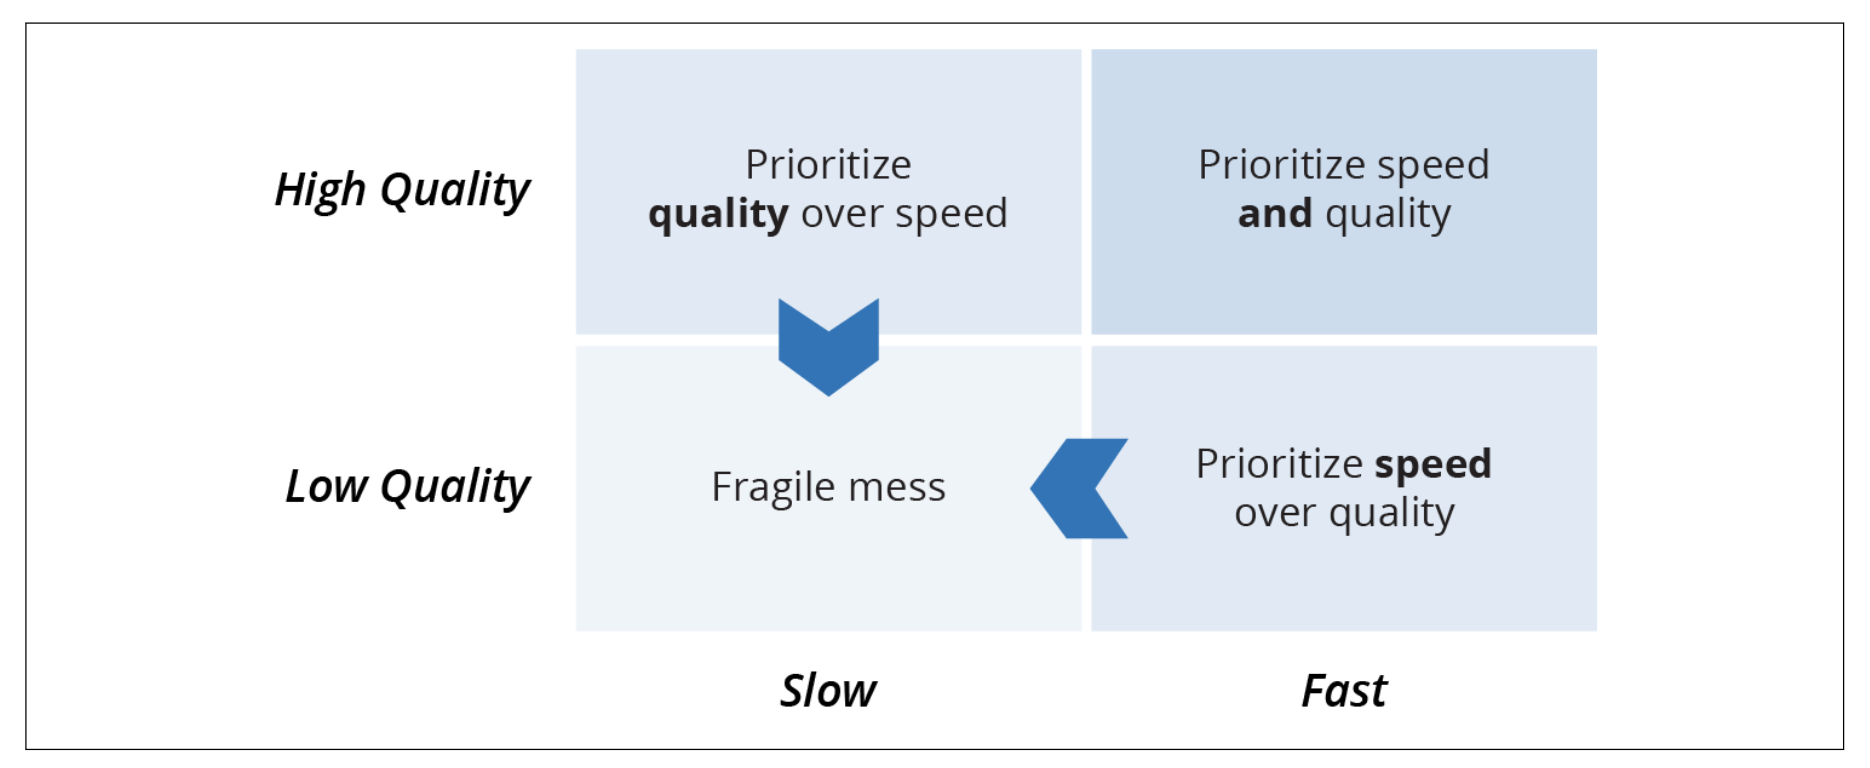
\includegraphics[width=1.0\textwidth]{fig/hauptteil/Speed_vs_Quality.png}
  \caption{Iron Age vs Cloud Age IaC Busch S.6}
  \centering
\end{figure}

Wird Geschwindgkeit über Qualität gestellt (Quadrant links oben) entstehen
mit der Zeit chaotische und instabiele Systeme an denen Veränderungen mit
der Zeit nur noch erschwert und deshalb langsam durchgeführt werden können.\\
Wird Geschwindigkeit zu niedrig priorisiert führt es allerdings auch dazu
dass letzten Endes durch Druck von Deadlines und schnellen workarounds
technische Schulden aufgebaut werden die ebenfalls zu einem qualitativ
schlechten System führen da notwendige Veränderungen nicht schnell genug
eingearbeitet werden können.

Aufgrund dieser Probleme ist es wichtig Geschwindgkeit und Qualität
gleichermaßen zu priorisieren, moderne Entwicklungsansätze DevOps
haben das Ziel dies zu erreichen, der Erfolg wird von der
Accelerate Studie belegt.

\subsection{Die drei Kernverfahren von IaC}

Kief Morris identifiziert drei Kernverfahren ("Core Practices")
zur Implementierung von Infrastructure as Code:

\begin{itemize} 
  \item \textbf{Define everything as Code:} Alle Teile eines System
  in Form von Code zu definieren bringt mehrere Vorteile mit sich.\\
  Code kann mehrfach ausgeführt werden, daher ist eine als Code
  definieres System Wiederverwendebar. Es können unkompliziert mehrere
  identische Instanzen erstellt werden, das Gilt auch für den Fall
  wenn Fehler auftreten und ein Neuaufbau erforderlich ist.
  Das Verhalten des Systems ist vohersehbar, fortlaufendes automatisches
  Testen ist möglich und damit auch zuverlässiger.\\
  Definition in Code macht auch den Aufbau eines Systems transparenter,
  da dieser immer dem tatsächlichen Zustand des Systems entspricht und
  damit auch dokumentiert.
  
  \item \textbf{Continuously Test and Deliver All Work in Progress:} 
  Fortlaufendes, automatisiertes Testen und Integrieren aller Komponenten
  die sich in Entwicklung befinden dient dem Ziel die Qualität eines
  Systems nicht nur "einzutesten" sondern von Beginn and und kontnuierlich
  einzubauen
  (The idea is to build quality in rather than trying to test quality in.
  (vgl IaC Buch S.10)). Nach der Accelerate Studie fördert es die Qualität
  der Arbeit eines Teams wenn jedes Mitglied mindestens einmal am Tag den
  eigenen Fortschritt integriert.

  \item \textbf{Build Small, Simple Pieces That You Can Change Independently:} 
  Systeme die aus mehreren kleineren voneinander unabhängigen Komponenten
  bestehen sind generell stabieler als große Monolithen. Eine Änderung die
  einen Fehler verursacht betrifft nur diese Komponente in der die Änderung
  stattfindet, diese kann dann leichter isoliert und das Problem behoben
  werden, kleine Komponenten sind in der Regel auch weniger Komplex und
  dadurch leichter zu verstehen. Ein einzelner Fehler nach einem Update
  hat auch den Vorteil dass nur diese Komponente und nicht das gesamte
  restliche System auf eine ältere Version zurückgesetzt werden muss um
  den Betrieb wieder herzustellen.

\end{itemize}

\subsection{Die Rolle von Terraform im IaC Anwendungsprozess}

Während der Anwendung von Infrastructure as Code kann primär zwischen zwei
wichtigen Phasen unterschieden werden, einer initialen Einrichtungsphase
und der darauf folgenden Wartungs- und Betriebsphase.\\
In der Einrichtung wird die Infrastruktur bereitgestellt und konfiguriert,
genauso wird auch Software intalliert und eingerichtet.\\
Nachdem das System dann in Betrieb genommen wurde können Anpassung notwendig
werden, Server werden hinzugefügt und abgebaut, Software wird aktualisiert
und neu konfiguriert.

\subsubsection{Überblick über die wichtigsten Infrastructure as Code Tools}

Infrastructre as Code beinhaltet verschiedene konkrete Anwendungsfälle und
entsprechend existieren auch Tools die zum Teil ein breiteres Spektrum
von IaC abdecken, zum Teil aber auch eher spezialisiert sind; Terraform
ist dabei ein Beispiel für ein spezialisierteres Tool. Die untenstehende
Abbildung soll einen Überblick über die aktuell relevantesten Tools
verschaffen, die Einordnungen sind dabei aber nicht unbedingt als absolut
anzusehen. Es ist zum Beispiel möglich innerhalb eines Terraform-Deployments
auch Software zu installieren und zu konfigurieren, allerdings wird die
tatsächliche Installation dann eher per von Terraform aufgerufenen Skripten
vorgenommen statt von Terraform selbst verwaltet zu werden, daher ist
Terraform hier ausschließlich als Infrastruktur-Management Tool eingeordnet.

\begin{figure}[H]
  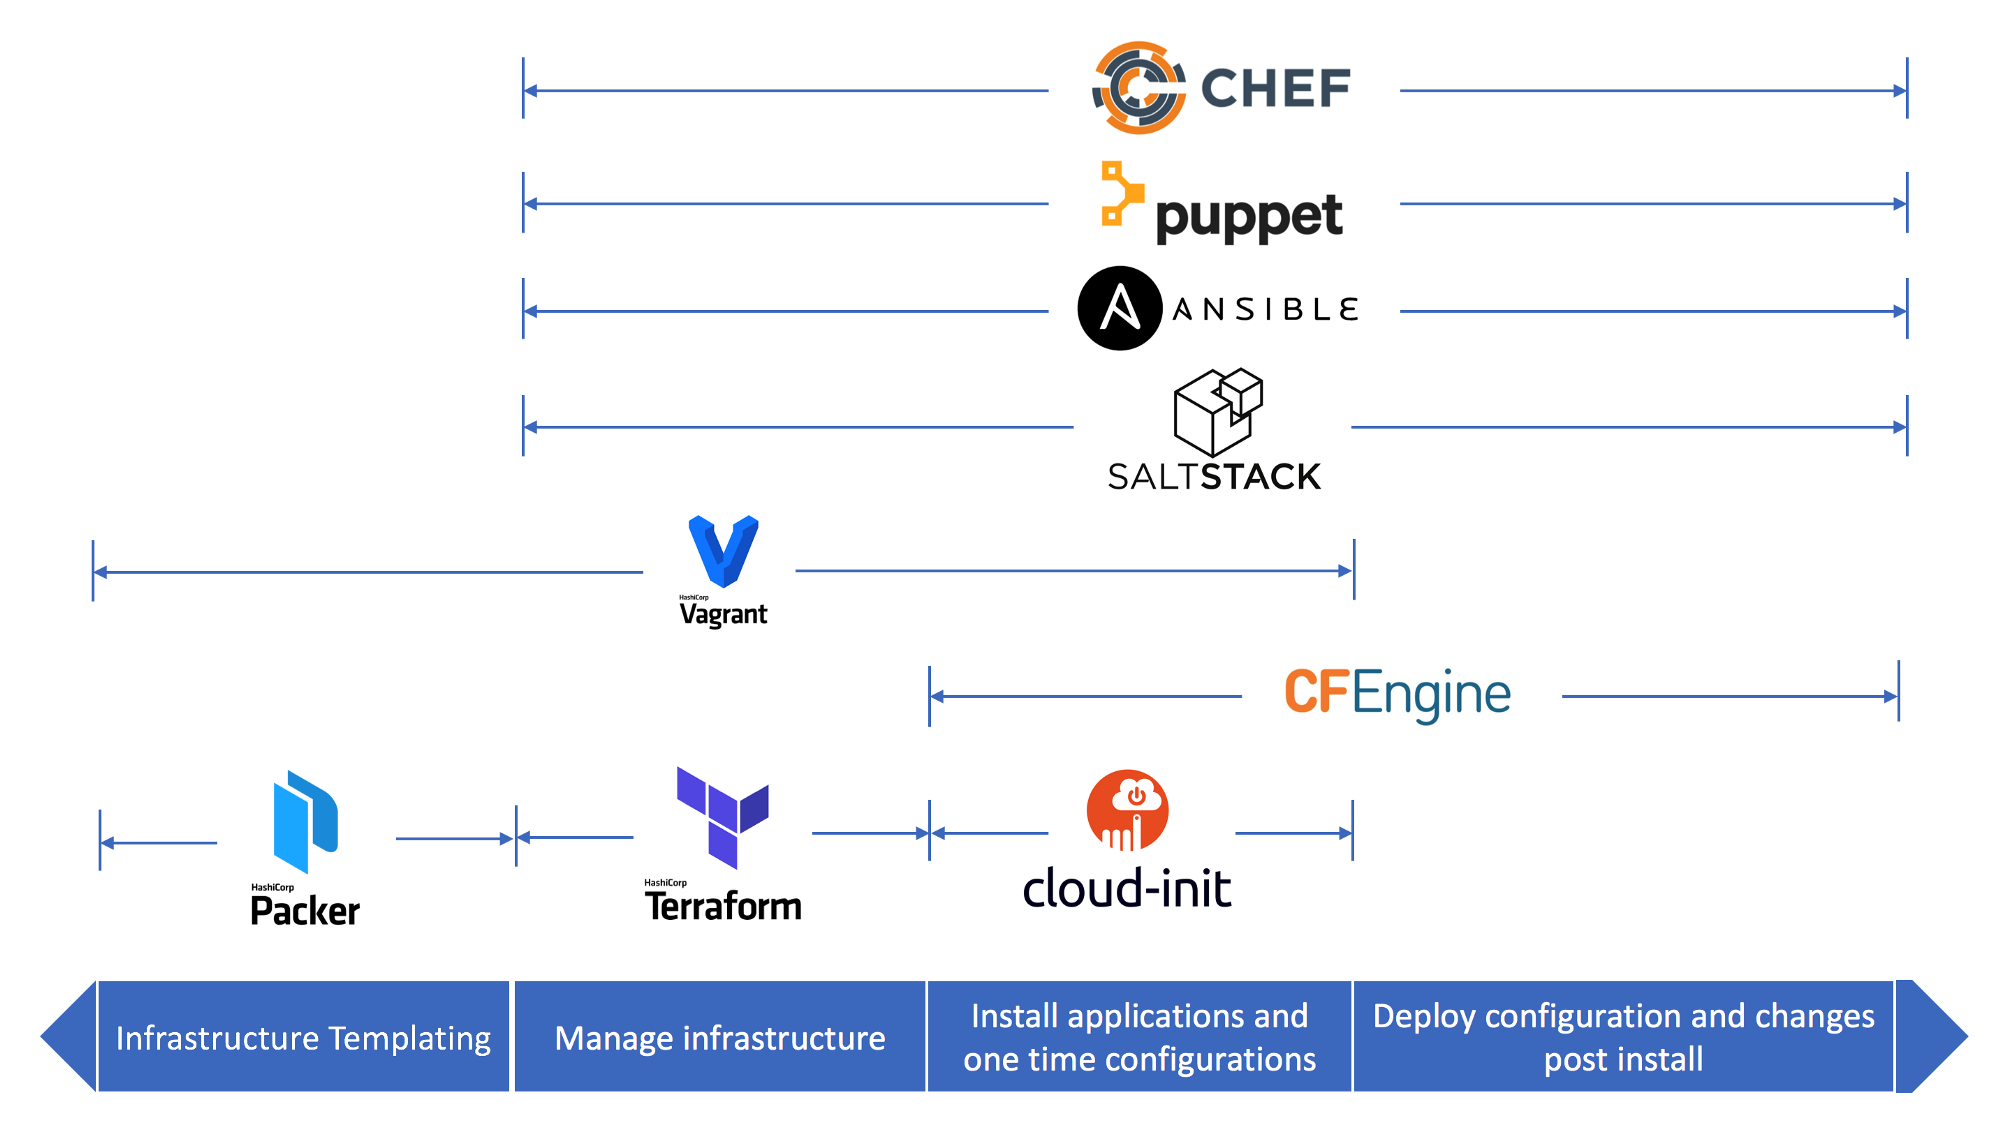
\includegraphics[width=1.0\textwidth]{fig/hauptteil/IaC_Tools.png}
  \caption{Überblick IaC Tools https://medium.com/cloudnativeinfra/when-to-use-which-infrastructure-as-code-tool-665af289fbde}
  \centering
\end{figure}

\subsubsection{Vorteile und Limiterungen von Terraform}

Da sich diese Arbeit primär mit dem Provisioning von grundlegender Cloud
Computing Infrastruktur in Form von VM's, Netzwerken, Datenspeicher und
anderen grundlegenden Komponenten beschäftigen soll bietet sich der Einsatz
eines darauf spezialisierten Tools an.\\
Hier gibt es zusätzlich zu Terraform eine weitere prominente Alternative:
Pulumi.

Pulumi bietet im Vergleich zu Terraform mehrere Vorteile, es gibt allerdings
auch diverse Nachteile die, gegen den Einsatz von
Pulumi sprechen. Die folgenden Vorteile bietet Pulumi gegenüber Terraform:

\begin{itemize}
  \item \textbf{Sprache:} Im Gegensatz zu Terraforms Domänen-spezifischer
  HashiCorp Configuration Language (HCL) setzt Pulumi auf den Einsatz
  bekannter General-Purpose Programmiersprachen, Python, TypeScript,
  JavaScript, Go, C\# und F\#, werden aktuell unterstützt.\\
  Durch den Einsatz dieser Sprachen können Schleifen, Funktionen und
  weitere bekannte Konstrukte verwendet werden, Terraform bietet diese
  Möglichkeiten nicht, ähnliche Effekte werden nur mit Workarounds erreicht.

  \item \textbf{Testing:} Um Terraform-code testen zu können werden
  Third-party Tools benötigt, Terraform selbst bietet kein Test-Framework.
  Durch den Einsatz bekannter General-Purpose Programmiersprachen in Pulumi
  ist es auch möglich die dort zum Einsatz kommenden Frameworks zu verwenden,
  Integrationstest sind allerdings nur in Go unterstützt
  (https://phoenixnap.com/blog/pulumi-vs-terraform).
  
  \item \textbf{Pulumi mit Terraform:} Pulumi kann kann sowohl lokale als auch
  remote Terraform State Files lesen und verarbeiten. Dies erlaubt es Pulumi
  und Terraform nebeneinander einzusetzen um verschiedene Teile der
  Infrastruktur mit dem jeweils anderen Tool zu managen, soll zum Beispiel 
  einer Umstellung von Terraform auf Pulumi erfolgen ist dies möglich
  ohne das gesamte System auf einmal auser Betrieb nehmen zu müssen.

\end{itemize}

Terraform wiederum bietet die folgenden Vorteile:

\begin{itemize}
  \item \textbf{Modularität:} Terraform Module erlauben es ein System in
  mehrere klar definierte Komponenten zu strukturieren, dadurch wird die
  Wiederverwendbarkeit dieser Komponenten ermöglicht und gefördert.
  Die daraus resultierenden Vorteile wurden bereits in den vorangegangenen
  Kapiteln dargelegt, daher soll hier nicht weiter darauf eingegangen werden.
  Pulumi strukturiert Infrastruktur Code entweder in einem großen
  monolithischen Projekt oder vielen kleinen Mikroprojekten, beide
  Optionen sind weniger flexibel als die Lösung die Terraform bietet.

  \item \textbf{State Debugging:} Es ist beinahe unvermeidbar
  dass es während der Arbeit an einem Infrastrukturprojekt über einen
  längeren Zeitraum irgendwann einmal zu einem Fehler im State kommt.
  Sowohl Terraform als auch Pulumi bieten hier CLI Befehle die bei der
  Fehlersuche und -behebung unterstützen, Terraform bietet hier jedoch
  aktuell noch mehr Optione mit denen Resourcen aus dem aktuellen State
  gelöscht oder hinzugefügt werden können, dadurch wird weniger händische,
  und potentiell fehleranfälligere Arbeit direkt im State File notwendig.

  \item \textbf{Weitere Verbreitung und größere Popularität:} Terraform wurde
  2014, Pulumi 2017 veröffentlicht, entsprechend ist Terraform deutlich weiter
  verbreitet und verfügt über all die Vorteile die eine größere Community mit
  sich bringt. Dazu gehören mehr Lernresourcen, mehr Codebeispiele, größere
  Bekanntheit und mehr Jobs für die Arbeit mit Terraform.

  \item \textbf{Dokumentation:} Einen weiteren Voteil von Terraform stellt
  dessen umfangreiche und ausgereifte Dokumentation sowie auch die
  Dokumentation der einzelnen Provider dar. Der genaue Aufbau der einzelnen
  Resourcen wie etwa einer VM auf Google Cloud Platform
  (google\_compute\_instance) ist mit einem Beispiel und der zugehörigen
  Argument Reference versehen aus der direkt ersichtlich wird welche
  Argumente notwendig (required), was der Zweck jedes einzelnen Arguments ist
  und wo anstelle eines einfachen Wertes ein Block erwartet wird.

\end{itemize}

-Terraform unterm Strich aktuell interessanter für große Projekte/Unternehmen
=> daher Wahl für diese Arbeit

- Ein wirklich fundierter Vergleich zwischen Terraform und Pulumi benötigt
deutlich mehr Zeit und Anspruch als im Rahmen dieser Arbeit möglich, für
die in diesem Fall und zu diesem Zeitpunkt zu treffende Entscheidung soll
der grobe Vergleich hier ausreichen. Ein umfangreicherer Vergleich zwischen
Terraform und Pulumi könnte in zwei Jahren ein anderes Ergebnis liefern
als heute, beide Technologien und insbesondere Pulumi sind noch relativ neu
und nicht vollständig ausgereift.

\subsubsection{Weitere zu beachtendende Aspekte}

Ein Aspekt über Terraform der häufig falsch interpretiert und verbreitet wird
ist dass Terrafom als Cloud agnostisch beschrieben ist. Dies ist NICHT der
Fall. Die einzelnen Terraform Provider welche jeweils die Abstraktion der
Cloud Service Provider tatsächlich vornehmen sind nicht austauschbar das heißt
der Terraform Code muss für jeden Cloud Service Provider individuell
geschrieben werden, Terraform Code ist daher nicht Cloud agnostisch.\\

(- Secrets Management? Terraform Enterprise?)

\subsection{Terraform Funktionsprinzip}

Terraform ist ein Infrastructure as Code Tool das es ermöglicht Infrastruktur
sicher und effizient aufzubauen, zu verändern und zu versionieren.\\
Terraform verwendet eine High-level DSL die es erlaubt die Infrastruktur in
deklarativer und menschenlesbaren Konfigurationsdateien zu beschreiben die
versioniert, geteilt und wiederverwendet werden können.\\
Bevor Veränderungen vorgenommen werden erzeugt Terraform einen Execution
Plan der beschreibt welche Veränderungen durchgeführt werden sollen und
überprüft werden kann bevor er ausgeführt wird.\\
Ein Resourcengraph der Abhängigkeiten erfasst erlaubt es voneinander
unabhängige Resourcen parallel und dadurch effizient zu erzeugen und gibt
einen besseren Einblick in den Aufbau des beschriebenen Systems.\\
Automatisierte Änderungen erlauben es komplexe Veränderungen an der
Infrastruktur mit minimaler menschlicher Interkation durchzuführen.
Terraform beachtet bestehende Abhängigkeiten und nimmt Veränderungen
durch Execution Plans schrittweise vor bis der definierte Zustand erreicht
ist. (Alles obere vgl https://www.terraform.io/intro/index.html)

Die folgende Abbildung stellt das Funktionsprinzip von Terraform mit den
wichtigsten beteiligten Komponenten dar.

\begin{figure}[H]
  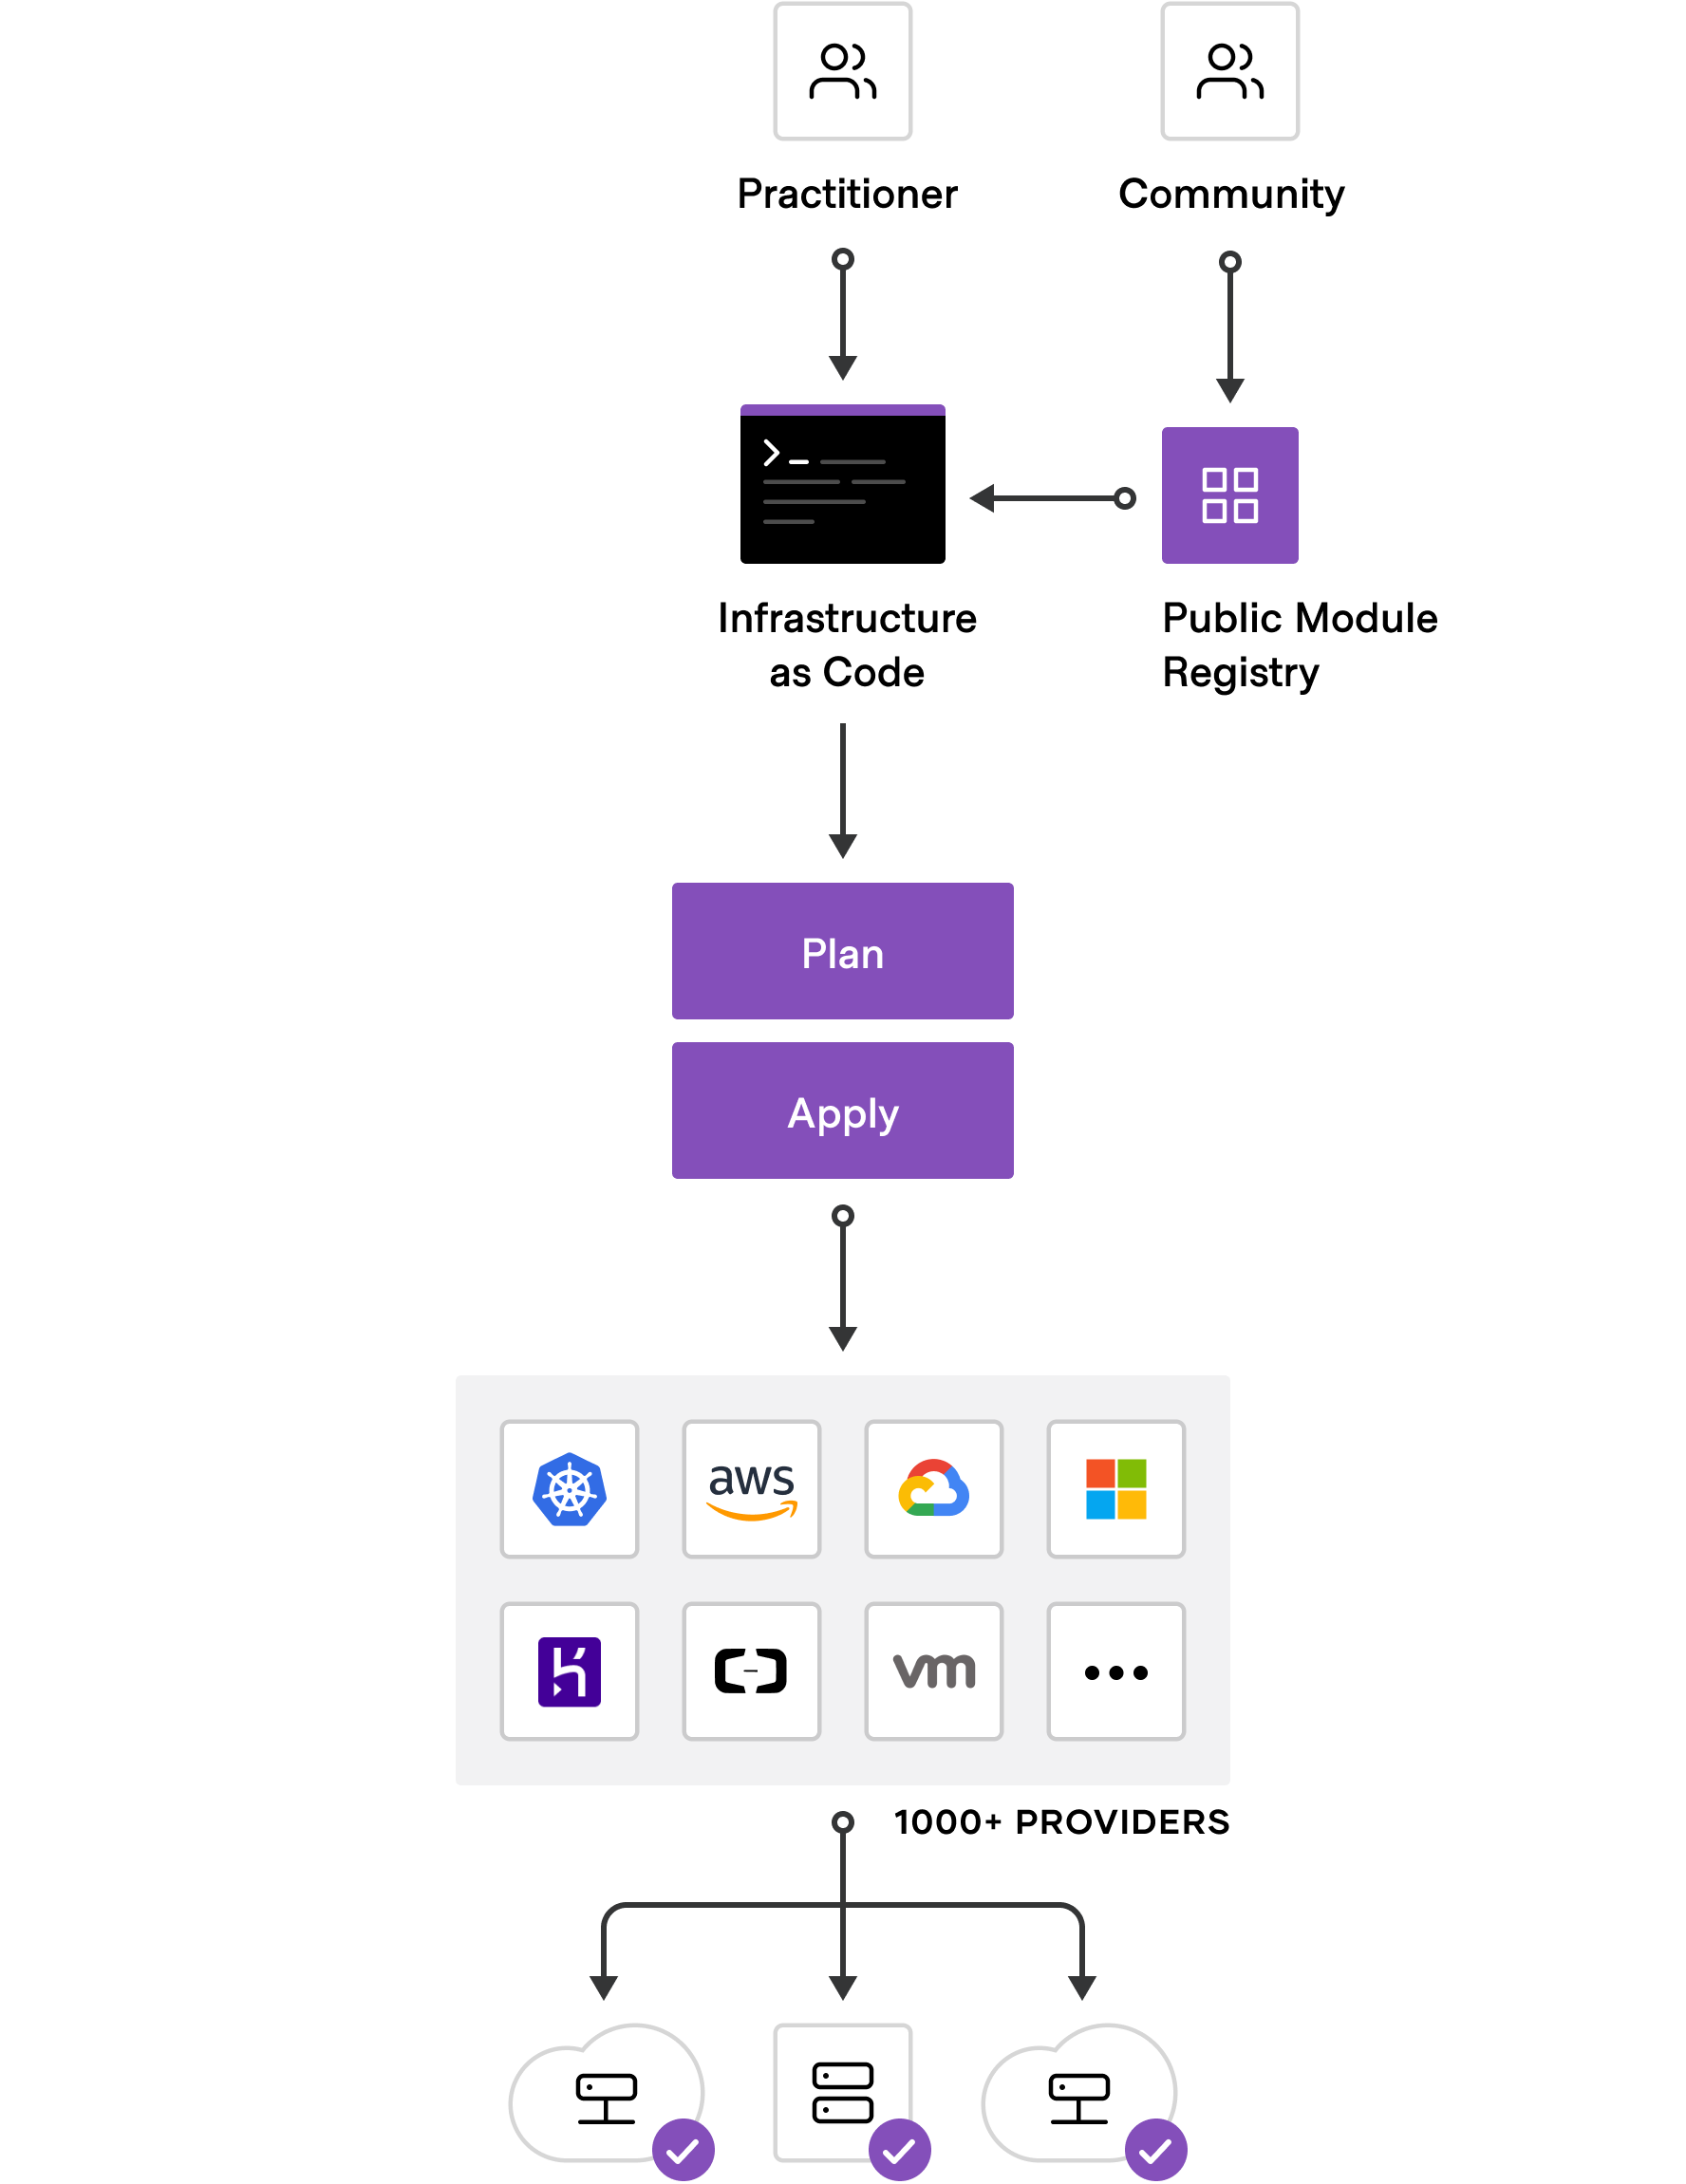
\includegraphics[keepaspectratio, height=15cm]{fig/hauptteil/Terraform.png}
  \caption{Terraform Funktionsprinzip}
  \centering
\end{figure}

Der Terraform Anwender schreibt den Infrastruktur Code in HCL. Dabei kann
er auf vorhandene Module aus der Public Module Registry zurückgreifen um
typische Strukturen wie Netzwerke aufzubauen. Die Terraform Core-Software
nutzt dann Plugins, die Terraform Provider, um die jeweiligen Cloud Plattform
API's anzusprechen die dann die Infrastrktur aufbauen. Die aktuell
existierenden Resourcen sind dabei in der terraform.tfstate Datei
festgehalten, gemeinsam mit dem aktuellen State und dem Infrastruktur Code
ermittelt Terraform welche Änderungen vorgenommen werden müssen um den
im Code beschriebenen Zustand zu erreichen.

\subsubsection{Hashicorp Configuration Language}

Die von Terraform verwendete Konfigurationssprache wurde mit dem Ziel
entwickelt einen Kompromiss zwischen Maschinenfreundlichkeit und
Menschenlesbarkeit zu erzielen. Existierende Serialisierungsformate,
Konfigurationssprachen und Programmiersprachen konnten die Ziele
der Terraform-Entwickler nicht erfüllen daher kommt nun bei Terraform
eine DSL in Form der Hashicorp Configuration Language zum Einsatz.

HCL besteht aus drei grundlegenden Elementen: Blöcken (Blocks), Argumenten
(Arguments) und Ausdrücken (Expressions).

TODO Codebeispiel

\textbf{Blöcke} stellen für gewöhnlich ein Objekt, im Fall von
Infrastrkturcode meistens eine Computing Resource, dar.
Blöcke besitzen einen Typ und Null bis mehrere label. Blöcke beinhalten
Argumente und weitere verschachtelte Blöcke.\\
\textbf{Argumente} sind das was in den meisten Programmiersprachen die
Variablen darstellen: Ein Wert der einem Namen zugewiesen wird.\\
\textbf{Ausdrücke} sind ähnlich wie in anderen Sprachen ein aus anderen
Ausdrücken und Argumenten berechneter Wert, ein Argument ist in diesem Sinne
die simpelste For eines Ausdrucks.

\subsubsection{Input und Output Variablen}

Input Variables sind nützlich um Parameter außerhalb des eigentlichen
Terraform Codes anzupassen. Die ID des Projektes stellt einen solchen
Parameter dar, befindet sich diese außerhalb des Codes muss nur die Datei
welche die Inputvariablen enthält angepasst werden, alles andere kann ohne
Veränderungen wiederverwendet werden.

TODO Codebeispiel

Inputvariablen sind einfache Key-Value Paare die einen Standardwert und
eine optionale Beschreibung besitzen.

Outputvariablen werden in der Regel verwendet um auf spezifische Parameter
einfachen und schnellen Zugriff zu ermöglichen.

TODO Codebeispiel

Werte wie die IP einer
Virtuellen Maschine auf einer Public Cloud Plattform sind vor der
Bereitstellung dieser nicht bekannt, werden aber häufig benötigt weshalb es
nützlich ist eine Output Variable für diese zu deklarieren.

\subsubsection{Terraform Module}

Module sind Container für mehrere Resourcen die gemeinsam verwendet werden.
Jedes Terraform Projekt besitzt ein Root Module das weitere Module verwenden
kann. Die Terraform Registry stellt eine Vielzahl an veröffentlichten
Modulen zur öfentlichen Verwendung bereit.

\subsubsection{Terraform Provider}

Terraform benötigt Plugins, die Provider, um mit Cloud Providern,
SaaS Providern und anderen API's interagieren zu können. (vgl https://www.terraform.io/docs/language/providers/index.html)
Provider ermöglichen es Terraform für gewöhnlich einen bestimmten Provider zu
konfigurieren, es gibt zum Beispiel einen Provider für Google Cloud
Platform, es gibt aber auch Provider die eine lokales Utility Tool für die
Nutzung durch Terraform konfigurieren. Öffentliche Provider werden primär
auf der Terraform Registry bereitgestellt und dokumentiert.

\subsubsection{Terraform Workflow}

Der grundlegende Terraform Workflow besteht aus vier Schritten:

TODO Code terraform init

Das init Kommando installiert und konfiguriert die notwendigen Provider
und Module und konfiguriert ein Backend (Fußnote Backend) falls angegeben.

TODO Code terraform plan

Mit terraform plan wird ein Execution Plan erstellt. Dazu gehört den die
aktuell existierenden Resourcen zu erfassen, Veränderungen zwischen
diesem Zustand und dem im Code konfigurierten Zustand zu erfassen und
auf Grundlage dessen einen Plan zu erstellen welche Änderungen vorgenommen
werden können um den Soll-Zustand zu erreichen.

Todo Code terraform apply

Durch terraform apply wird ein solcher Execution Plan ausgeführt und die darin
enthaltenen Änderungen an der Infrastruktur vorgenommen.

Todo Code terraform destroy

Um den umkomplizierten Abbau eines mit Terraform definierten und aufgebauten
Systems bewerkstelligen zu können wird das terraform destroy Kommando
verwendet. Dies ist besonders nützlich um nicht mehr benötigte Testsysteme
und andere temporäre Infrastrukturen zu entfernen.

\chapter{Aufbau und Untersuchung}
\label{sec:real}

\section{Evaluierungsanforderungen}

\subsection{Ziel der Evaluierung}

Das Ziel der Evaluierung ist es einen Vergleich zwischen den Terraform
Providern von Amazon AWS, Google Cloud Platform und Microsoft Azure zu
erstellen. Der Hintergrund dazu ist es als erstes zu ermitteln ob alle
drei der großen Cloud Plattformen Infrastructure as Code mit Terraform
für ein gegebenes Szenario unterstützen. Weiter sollen mehrere
Kriterien verglichen werden um zu ermitteln ob alle Plattformen
vergleichbare Ergebnisse liefern, oder ob eine Plattform durch besonders
gute oder schwache Ergebnisse heraussticht. Funktionieren bestimmte
Aspekte (wie zum Beispiel die Containerimage-Registry) unterschiedliche
soll dies ebenfalls erfasst und bewertet werden.\\
Die Untersuchung soll auch dazu dienen die Effektivität von
Infrastructure as Code mit Terraform zu demonstrieren. Zusätzlich soll
dargestellt werden dass die Technologie einsatzreif für Verwendung in
Produktionssystemen ist.

\subsection{Zu untersuchende Komponenten der Terraform Provider}

Die Komponenten der Terraform Provider die Untersucht werden sollen
hängen von dem System ab das als Untersuchungsobjekt genutzt werden soll.
Dieses setzt sich aus einem Netzwerk, einer Container-Registry, einem
Kubernetes-Cluster und einem Datenbankserver mit mehreren Datenbanken
sowie den dazugehörenden Firewalls zusammen. Zusätzlich sollen
einfache virtuelle Maschinen betrachtet werden um ein vollständigeres Bild
zu erhalten.

\subsection{Grenzen und Limitierungen der Evaluierung}

Die Terraform Provider können weitaus mehr Computing Ressourcen erzeugen
als in dieser Arbeit untersucht werden. Aufgrund des Umfangs können
nicht alle Ressourcen verglichen werden, die hier verwendeten wurden
ausgewählt um die grundlegendsten Szenarien zu untersuchen. Da die durch
die verschiedenen Cloud Provider bereitgestellten Computing Ressourcen
jedoch
nicht immer identisch sind ist ein perfekter Vergleich nicht möglich.
Stellen die Cloud Provider nur Virtuelle Maschinen mit unterschiedlicher
Leistungsfähigkeit bereit wird jedoch darauf geachtet möglichst ähnliche
Konfigurationen zu verwenden um den Vergleich so identisch wie möglich zu
gestalten. Das selbe gilt für die Größen von Festplatten und allen anderen
vergleichbaren Objekten. Stehen nur sehr teure identische Maschinen bereit
werden aus Kostengründen ebenfalls günstigere aber möglichst ähnliche
Konfigurationen gewählt. Die genauen Daten der verglichenen
Infrastrukturobjekte werden jeweils bei den Vergleichswerten aufgelistet.

\section{Spezifizierug des Vergleichs}

\subsection{Auswahl der zu untersuchenden Aspekte und Eigenschaften}

Das Softwarequalitätsmodell der ISO 25010 wird als ein Grundstein für die
Evaluierung von Software beschrieben (Vergleich https://iso25000.com/index.php/en/iso-25000-standards/iso-25010)
Da die Terraform Provider statt einer ganzheitliche Software nur Plu-Ins
und damit eine kleinere Komponente von Terraform darstellen kann nicht
jeder der in der ISO 25010 aufgelistet Punkte sinnvoll angwendet werden.
Einige Bereiche, zum Beispiel der Bereich Security mit all seinen
untergeordneten Themen, benötigen eine deutlich genauere Betrachtung als
es im Rahmen dieser Arbeit möglich ist um ein sinnvolles und vollständiges
Ergebnis gewährleisten zu können.\\
Aus diesem Grund sollen nur ein kleinerer Teil der aufgeführten Merkmale
betrachtet werden, interessant sind vor allem solche die eine schnelle
Einführung von Terraform in den Entwicklungsprozess beeinflussen.
Ebenfalls interessant sind die Flexibilität und Wartbarkeit da
insbesondere letztere einen der großen Vorteile darstellt die man durch
den Einsatz von Infrastructure as Code Tools- und Prinzipen erzielen kann.

\begin{figure}[H]
  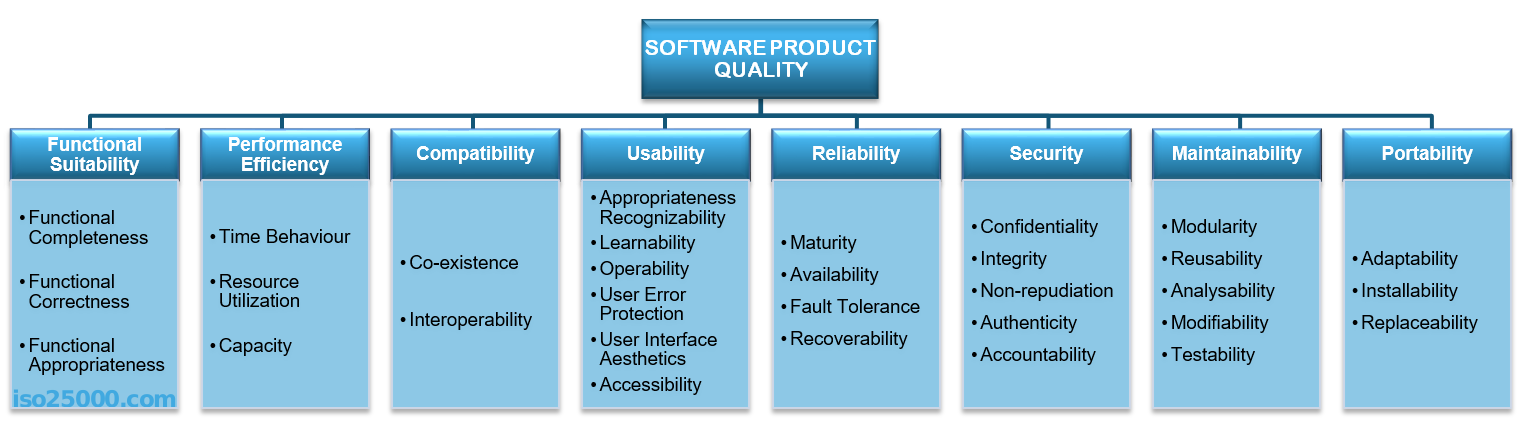
\includegraphics[keepaspectratio, height=4.5cm]{fig/hauptteil/ISO25010.png}
  \caption{Überblick ISO 25010}
  \centering
\end{figure}

Im Folgenden sollen die einzelnen Merkmale der ISO 25010 kurz
zusammengefasst werden und erläutert werden ob diese in der Evaluierung
der Terraform Provider sinnvoll betrachtet werden können und ob eine
Betrachtung im Rahmen dieser Arbeit vorgenommen werden kann.

\subsubsection{Functional Suitability}

\begin{itemize}
  \item \textbf{Functional completeness}: Die Vollständigkeit mit welcher
  die Aufgaben und Ziele die vom Nutzer an die Software gestellt werden
  erfüllt werden können.

  Anwendbarkeit: Eine zufriendenstellende Functional Completeness ist die
  grundlegende Vorraussetzung für den Einsatz jeder Software, dies gilt
  auch für den Einsatz von Terraform und die zu untersuchenden Provider.

  \item \textbf{Functional correctness}: Grad zu welchem die Software
  korrekte Ergebnisse mit einer ausreichenden Genauigkeit liefert.

  Anwendbarkeit: Da im Falle der Bereitstellung von Infrastruktur durch
  deklarativen Code wenig Spielraum zulässt und im Fall der hier
  untersuchten Systeme lediglich ein \enquote{richtig} oder
  \enquote{falsch} zulässt spielt dieser Punkt keine Rolle.

  \item \textbf{Functional appropriateness}: Grad zu welchem die
  Funktionalitäten der Software die Erfüllung der Aufgaben ermöglichen
  und unterstützen.

  Anwendbarkeit: Da die Terraform Provider im Prinzip nur eine
  Schnittstelle zu den jeweiligen Plattformen darstellen ist dieser Aspekt
  hier wenig relevant. Bei einer allgemeinen Betrachtung der
  Funktionalität von Terraform wäre dieser Punkt jedoch sehr interessant.
\end{itemize}

\subsubsection{Performance Efficiency}

\begin{itemize}
  \item \textbf{Time behaviour}: Grad zu welchem die Anforderungen an
  Bearbeitungszeit und Durchsatz erfüllt werden.

  Anwendbarkeit: Die Dauer in welcher ein System von der Plattform durch
  den jeweiligen Terraform Provider bereitgestellt werden kann ist ein
  relevanter Aspekt der sehr gut untersucht und verglichen werden kann.

  \item \textbf{Resource utilization}: Beschreibt Umfang und Typ der
  Ressourcen die von der Software während des Betriebs benötigt werden.

  Anwendbarkeit: Da die Terraform Provider selbst nur die
  Schnittstelle darstellen ist dieser Aspekt nicht sinnvoll anwendbar.
  Bei einem
  Vergleich verschiedener Softwaretools wäre dieser Aspekt von größerer
  Bedeutung.

  \item \textbf{Capacity}: Grad zu welchem die maximalen Limits der
  Software die Anforderungen erfüllen.

  Anwendbarkeit: Auch dieser Aspekt ist nicht relevant, es trifft die
  die selbe Argumentation wie beim vorhergehenden Punkt zu.
\end{itemize}

\subsubsection{Compatibility}

\begin{itemize}
  \item \textbf{Co-existence}: Grad zu welchem die Software ihre Funktion
  erfüllen kann während sie sich eine Umgebung mit anderen Programmen
  teilt ohne deren Funktionalität zu beeinträchtigen.

  Anwendbarkeit: Da in diesem Bereich im Rahmen der Arbeit mit wenigen
  Providern keine Probleme zu erwarten sind wird dieses Thema nicht
  explizit betrachtet.

  \item \textbf{Interoperability}: Grad zu welchem die Software mit
  anderen Produkten Informationen austauschen und verarbeiten kann.

  Anwendbarkeit: Im Rahmen der Arbeit wird die Interaktion zwischen
  den Providern von Google Coud Platform und Microsoft Azure mit
  Kubernetes und Helm betrachtet.
\end{itemize}

\subsubsection{Usability}

\begin{itemize}
  \item \textbf{Appropriateness recognizability}: Beschreibt wie einfach
  ein Nutzer erkennen kann ob die Software eine angemessene Lösung für
  dessen Anwendungsfall darstellt.

  Anwendbarkeit: Dieser Aspekt kann zu einem gewissen Grad betrachtet
  und bewertet werden. Die Bezeichnungen der verschiedenen Computing 
  Ressourcen können zum Beispiel ihre Funktion gut oder auch weniger
  genau beschreiben.

  \item \textbf{Learnability}: Grad zu welchem ein bestimmter User
  bestimmte Lernziele in einem definierten Kontext erreichen kann.

  Anwendbarkeit: Eine Untersuchung der Erlernbarkeit eines Terraform 
  Providers könnte durchaus vorgenommen werden. Um ein aussagekräftiges
  Ergebnis erzielen zu können wären jedoch umfangreichere Untersuchungen
  mit mehreren Usern notwendig weshalb im Rahmen dieser Arbeit dieses
  Kriterium nicht betrachtet werden soll.

  \item \textbf{Operability}: Beschreibt Attribute die ein System besitzt
  das dessen Bedienung vereinfacht.

  Anwendbarkeit: Bei einer Betrachtung von Terraform als ganzes könnte
  dieser Punkt sinnvoll untersucht werden, die einzelnen Provider
  unterscheiden sich hier jedoch nicht.

  \item \textbf{User error protection}: Grad zu dem die Software den
  Nutzer gegen eigene Fehler (z.Bsp. während der Eingabe) schützt.

  Anwendbarkeit: Hier liegt die selbe Lage wie beim vorhergehenden
  Punkt vor, wird daher nicht betrachtet.

  \item \textbf{User interface aesthetics}: Beschreibt wie ansprechend
  und zufriedenstellend das Userinterface bewertet werden kann.
  
  Anwendbarkeit: Dieser Aspekt ist irrelevant da die Terraform Provider
  nicht direkt verwendet werden und kein User interface besitzen.
  Terraform selbst wird aus der Kommandozeile heraus bedient.

  \item \textbf{Accessibility}: Grad zu welchem die Software von
  verschiedenen Nutzern mit verschiedenen Fähigkeiten und Charakteristiken
  verwendet werden kann.

  Anwendbarkeit: Für den Vergleich der Provider nicht anwendbar. Die 
  selbe Argumentation wie bei Operability und User error protection
  treffen auch hier zu. 
\end{itemize}

\subsubsection{Reliability}

\begin{itemize}
  \item \textbf{Maturity}: Beschreibt wie zuverlässig die Software unter
  normalen Bedingungen arbeitet.

  Anwendbarkeit: Durch den begrenzten Umfang der in dieser Thesis
  durchgeführten Arbeiten kann dieser Aspekt nur begrenzt betrachtet
  werden. Sollten Auffälligkeiten in diesem Bereich auftreten werden
  diese jedoch erfasst und dokumentiert.

  \item \textbf{Availability}: Beschreibt ob die Software betriebsbereit
  und verfügbar ist.

  Anwendbarkeit: Da die Terraform Provider nur ein Plug-In darstellen
  hängt dieser Aspekt sowohl von Terraform und den Cloud Plattformen ab,
  nicht von den Providern selbst.

  \item \textbf{Fault tolerance}: Grad zu welchem die Software trotz
  Hard- und Softwarefehlern ihre Funktion erfüllen kann.

  Anwendbarkeit: Auch dieses Kriterium ist beim Vergleich zwischen den
  Providern nicht von Bedeutung da die Funktionalität nicht von diesen
  abhängt.

  \item \textbf{Recoverability}: Grad zu welchem die Software bei einger
  Unterbrechung oder einem Fehler betroffene Daten widerherstellen und
  die Funktionalität widerherstellen kann.

  Anwendbarkeit: Hier kann untersucht werden ob Terraform bei
  den veschiedenen Providern unterschiedlich auf einen Abbruch der 
  Internetverbindung oder bei einer fehlerhaften Eingabe reagiert.

\end{itemize}

\subsubsection{Security}

Das Thema Security beinhaltet die Merkmale Confidentiality, Integrity,
Non-repudiation, Accountability und Authenticity. Auf die
Sicherheit von Terraform und den jeweiligen Coud Plattformen soll
aufgrund des Umfangs und der Komplexität des Themas im Rahmen dieser
Arbeit nicht eingegangen werden. Für einen Vergleich der Terraform
Provider selbst ist das Thema ohnehin weniger von Interesse da die
Sicherheit stärker von Terraform selbst und den einzelnen Cloud
Plattformen abhängt als von den individuellen Providern. 

\subsubsection{Maintainability}

\begin{itemize}
  \item \textbf{Modularity}: Beschreibt den Grad zu welchem ein System 
  voneinander unabhängigen Komponenten aufgebaut ist.

  Anwendbarkeit: Dieser Aspekt wird von Terraform selbst implementiert
  und spielt bei der Betrachtung verschiedener Provider keine Rolle.
  Interessant wäre jedoch ein Vergleich zwischen Terraform und anderen
  IaC Tools welcher im Rahmen dieser Arbeit jedoch nicht vorgenommen wird.

  \item \textbf{Reusability}: Beschreibt wie gut sich Komponenten in
  anderen Systemen und Komponenten wiederverwenden lassen.

  Anwendbarkeit: Auch dieser Aspekt ist für den Vergleich nicht
  relevant, die Argumentation ist die selbe wie für das Thema Modularity.
  Für einen Vergleich mit anderen Tools wäre dies ein sehr relevantes
  Thema da Terraform sehr gute Optionen besitzt um das Schreiben
  modularen Codes zu fördern. 

  \item \textbf{Analysability}: Grad der Effektivität und Effizienz mit
  der der Einfluss auf das System ermittelt werden kann der durch eine
  Veränderung verursacht wird. Dazu gehört auch das Ermitteln von 
  Komponenten die verändert werden sollen sowie das diagnostizieren von
  Fehlern und Schwächen des Produkts.
  
  Anwendbarkeit: Analysability ist ein Aspekt der sowohl
  von Terraform selbst als auch von der Cloud Plattform abhängt. Dieses
  Thema soll im Rahmen dieses Vergleichs nicht betrachtet werden da
  es zu großen Teilen nicht vom Provider abhängt.
  
  \item \textbf{Modifiability}: Beschreibt wie gut ein System verändert
  werden kann ohne Fehler aufzuwerfen oder die Qualität zu verschlechtern.

  Anwendbarkeit: Hier kann untersucht werden ob es im Fall der
  Modifizierung von einzelnen Ressourcen Unterschiede gibt. Es kann
  untersucht werden ob bei den Plattformen Ressourcen bei einer
  vergleichbaren Modifikation gelöscht und neu erstellt werden oder
  ob ein stoppen, verändern und neu starten ausreicht bzw. die
  Eigenschaft im laufenden Betrieb mit minimaler Unterbrechung des
  Services verändert werden kann. 
  
  \item \textbf{Testability}: Effektivität und Effizienz mit der
  Testkriterien etabliert werden und entsprechende Tests durchgeführt
  werden können.

  Anwendbarkeit: Im Vergleich der Provider ist das Thema Testen
  weitgehend irrelevant. Sehr interessant wäre jedoch wieder der Vergleich
  mit anderen vergleichbaren Tools, Terraform selbst beinhaltet
  wenig bis keine Möglichkeiten für Test und setzt mehr auf zusätzliche
  Tools und Frameworks.
\end{itemize}

\subsubsection{Portability}

Portability fasst die Aspekte Adaptability Installability und
Replaceability zusammen. Bei einem Vergleich der Terraform Provider
können diese Aspekte nicht sinnvoll miteinander verglichen werden da
diese von Terraform selbst und nicht von den Providern abhängen.


\subsubsection{Zusammenfassung der für den Vergleich ausgewählten Aspekte}

Für den im Rahmen dieser Arbeit durchgeführten Vergleich werden nur
einige der in der ISO 25010 definierten Qualitätsmerkmale betrachtet.
Da die Terraform Provider nur einen Teil der gesamten Software ausmachen
sind zahlreiche Aspekte kaum oder gar nicht von den Terraform Providern
abhängig und werden aus diesem Grund nicht betrachtet, andere Themen
sind zu umfangreich und/oder komplex um hier zufriedenstellend
bewertet werden zu können.\\
Kurz zusammengefasst werden die folgenden Merkmale betrachtet:

\begin{itemize}
  \item \textbf{Functional completeness}
  \item \textbf{Time behaviour}
  \item \textbf{Recoverability}
  \item \textbf{Modifiability}
\end{itemize}

\subsection{Entscheidungskriterien für die Evaluierung}

Da im Falle dieser Arbeit ein Vergleich ohne bestimmte quantitative
Ziele vorgenommen wird werden hier keine spezifischen
Entscheidungskriterien wie in der ISO 25040 beschrieben. Stattdessen
soll betrachtet werden wie die drei Provider in Relation zueinander
abschneiden. Dadurch kann ermittelt werden ob ein Provider den anderen
in bestimmtem Bereichen überlegen ist, ob sich zum Beispiel das
zeitliche Verhalten wesentlich unterscheidet oder ob ein Provider
grundlegende Bedingungen wie die funktionale Vollständigkeit nicht
aufweist.\\
Die gemessenen Werte und andere auffallende Merkmale sollen jeweils
tabellarisch dargestellt werden um die Übersichtlichkeit zu fördern
und Unterschiede der Provider leicht einsehbar zu machen.

\section{Umsetzung}

\subsection{Eingesetzte Software und Tools}

In diesem Abschnitt sollen die Tools die bei der Umsetzung zum Einsatz
kommen knapp zusammengefasst werden.

Als Source-code Editor kommt Visual Studio Code zum Einsatz.\\
Die Versionierung des Source-codes erfolgt durch ein privates
Git-Repository auf Github.\\
Github Actions wird eingesetzt um Änderungen
am Infrastruktursystem automatisch durchzuführen. Um das automatische
Deployment der Infrastruktur zu ermöglichen werden die dafür notwendigen
Secrets als Github Actions Secrets direkt im Repository gespeichert.\\
Zeitmessungen werden mit dem Bash Kommando \textbf{time <command>}
durchgeführt und das Ergebnis der Zeile \textbf{real} verwendet.\\
Terraform und Terraform Provider kommen in den jeweils im Source-code
definierten Versionen zum Einsatz.

\subsection{High-level Aufbau der Infrastruktur des Versuchsobjekts}

Als primäres Testobjekt dient ein Infrastruktursystem das typische Anwendungsfälle
repräsentieren soll. Es besteht aus Netzwerk, mehreren Datenbanken und 
einem Kubernetes Cluster mit mehreren Worker Nodes. Das System ist eine
leicht veränderte Variante des öffentlich einsehbaren
Infrastruktur-Showcase der Novatec.\\
Weiterhin existiert ein bereits manuell erstellter Object Storage mithilfe
dessen auf einer ebenfalls manuell erstellten Container Registry das
Dockerimage für den Kubernetes Cluster bereitgestellt wird. Dieses Image
bzw. die Registry wird dann im Terraform Projekt als Data Source erfasst.\\
Ergänzend zu diesem System sollen 
zusätzlich einige Tests mit einzelnen Ressourcen wie zum Beispiel
Virtuellen Maschinen durchgeführt werden.

Der originale Infrastrktur-Showcase besteht aufgrund der verhältnismäßig
geringen Größe und Komplexität aus einem einzelnen Terraform Modul
"Platform" das die gesamte Infrastruktur enthält. Für diese Arbeit wurden
die Kubernetes- und Datenbank-Komponenten zu Demonstrationszwecken in
jeweils eigene Module ausgelagert. Diese Module könnten in
eine öffentliche oder auch private Terraform Module Registry
hochgeladen werden um später in weiteren Projekten verwendet werden zu
können.

\begin{figure}[H]
  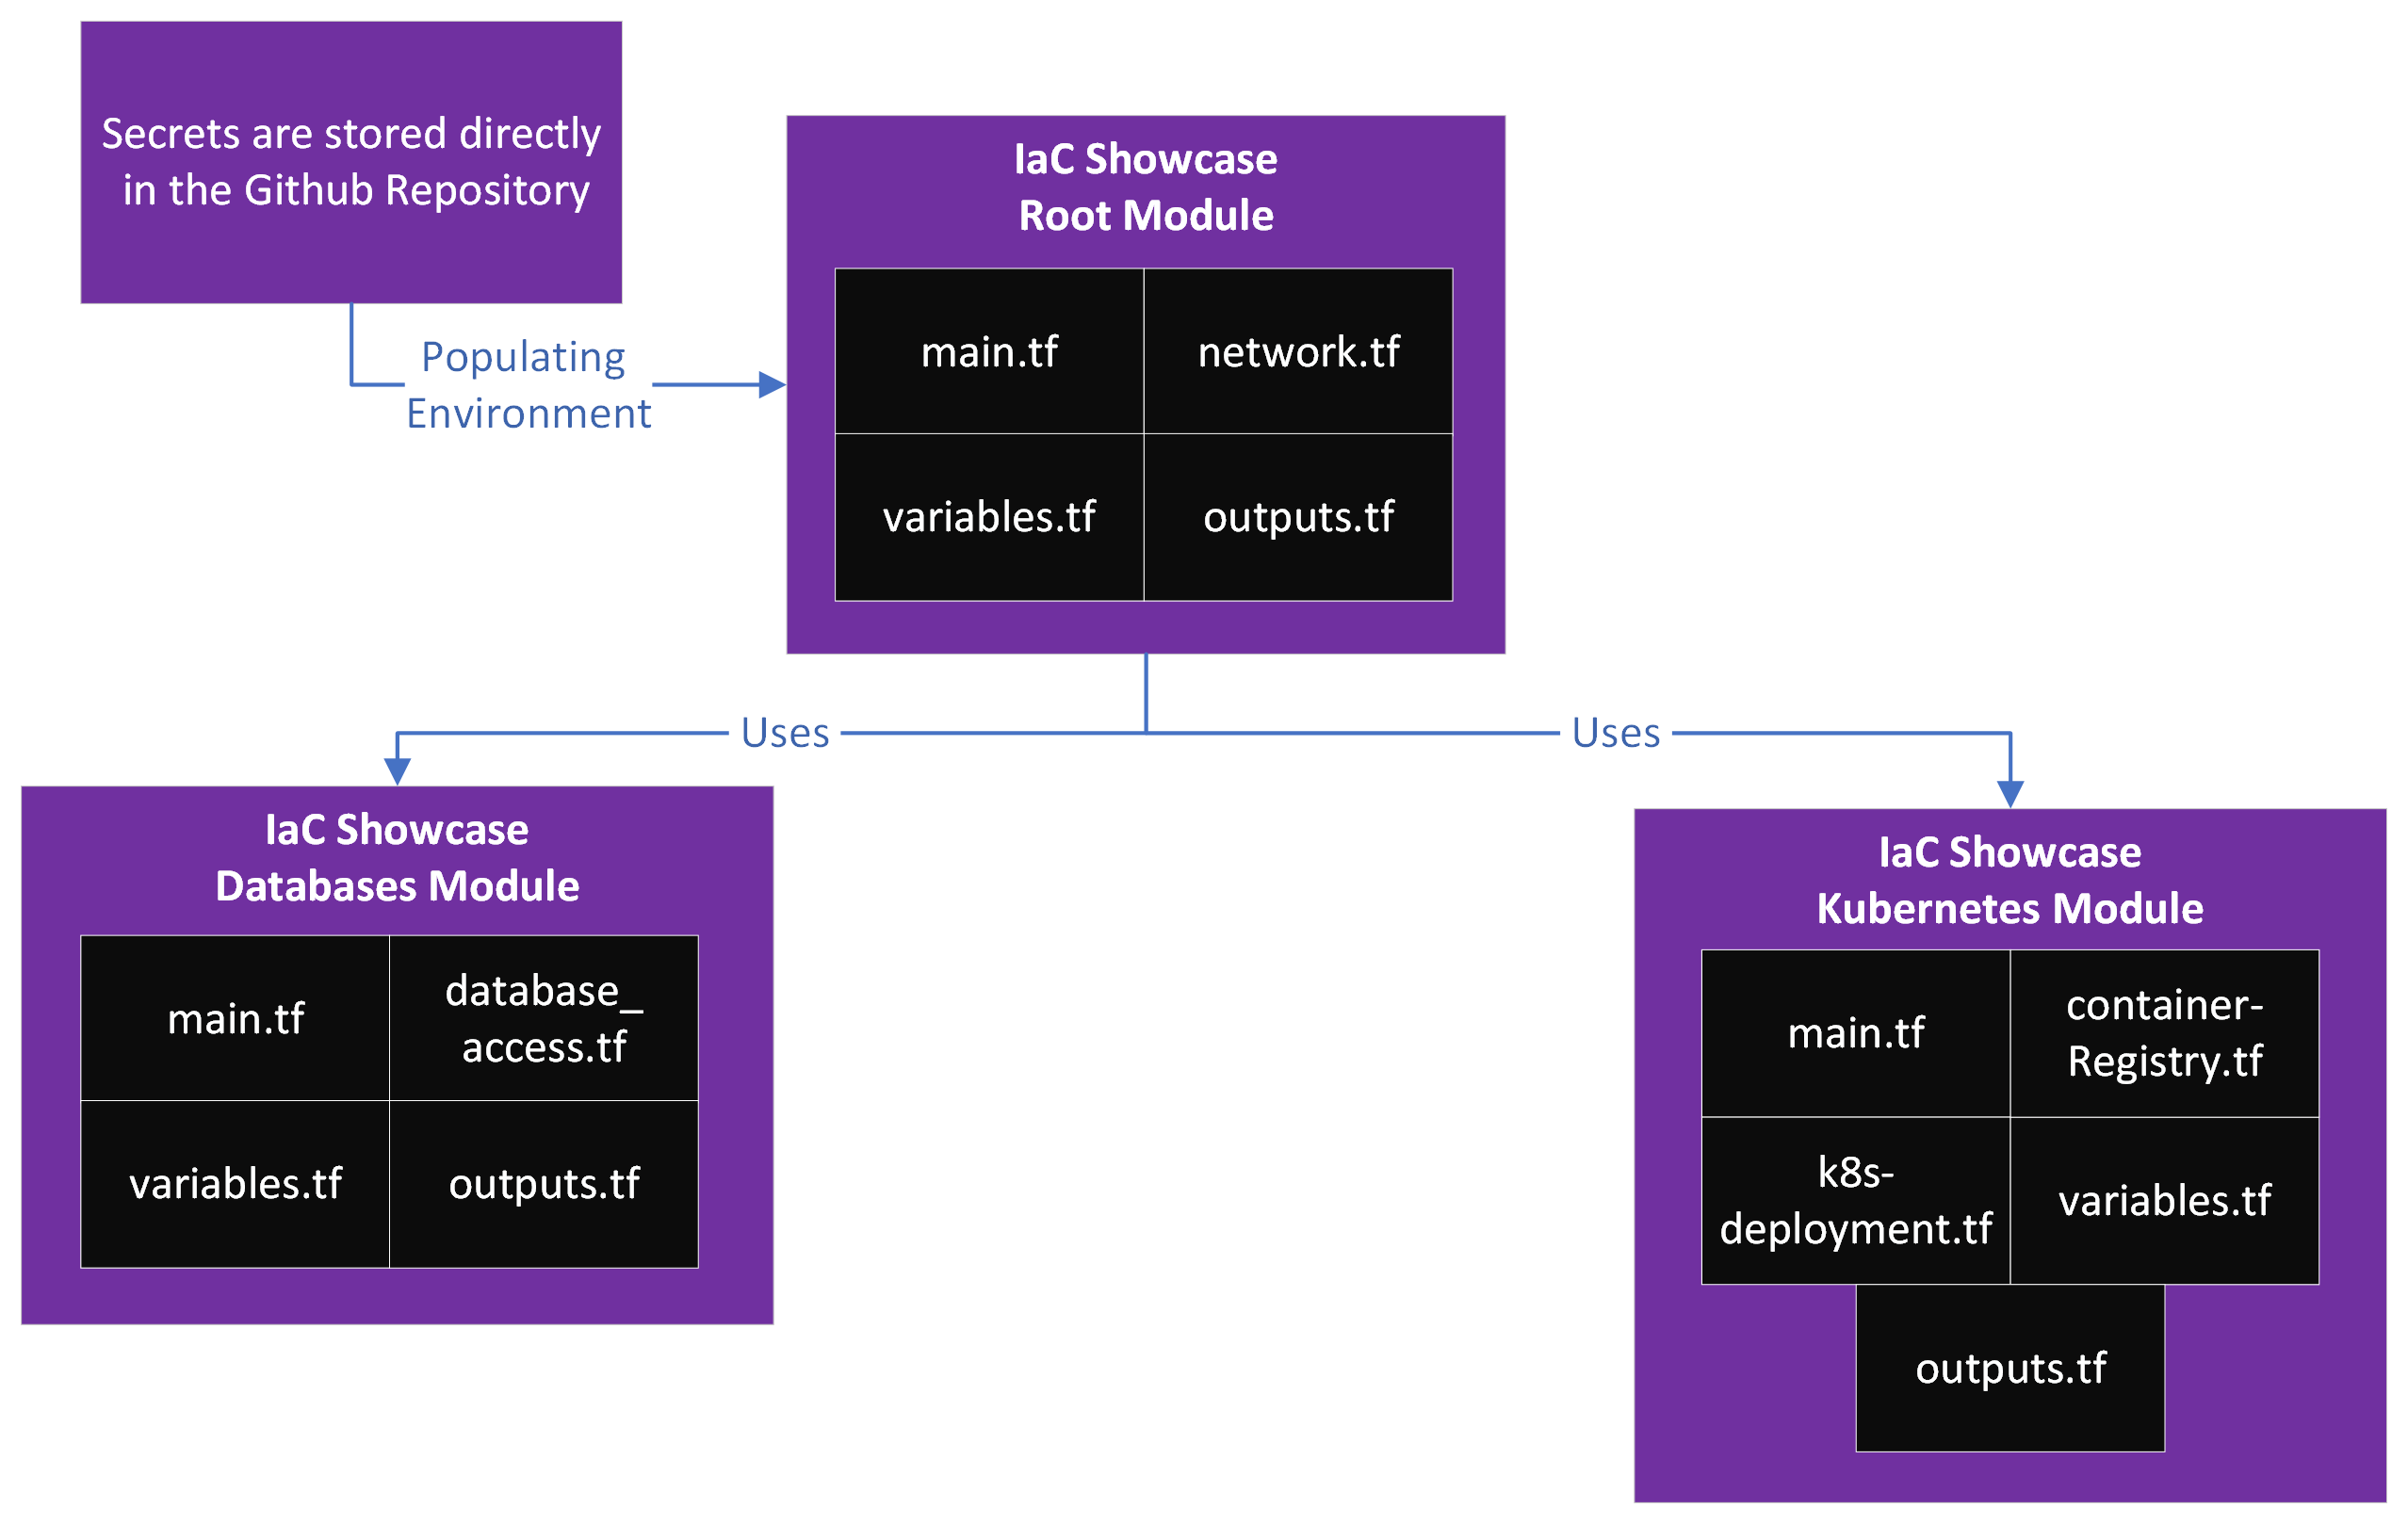
\includegraphics[keepaspectratio, height=10cm]{fig/hauptteil/IaC_Showcase_Structure_High-level.png}
  \caption{Infrastructure Showcase High-level Struktur}
  \centering
\end{figure}

In der Abbildung der High-level Struktur wird auf eine detaillierte
Darstellung der Ressourcen verzichtet da je nach Plattform verschiedene
Funktionalitäten in unterschiedlichen Ressourcen zusammengefasst werden
können. Stattdessen wird durch .tf-Dateien dargestellt welche
Funktionalität in in welchem Modul vorhanden sein soll und wie der Code
des Systems in Hinsicht auf Dateien aufgeteilt werden soll.

\subsection{Konkreter Aufbau der Versuchssysteme}

Im folgenden Unterkapitel werden die konkreten Aufbauten der Systeme
dargestellt. Die Diagramme der Systeme wurden mithilfe des in
terraform integrierten \textbf{terraform graph} erstellt und im
Anschluss dem externen Tool \textbf{Terraform Graph Beautifier}
visuell aufbereitet. In den Diagrammen sind jeweils alle Ressourcen
der Systeme sowie alle Variablen, Outputs und deren Abhängigkeiten
dargestellt.

\begin{figure}[H]
  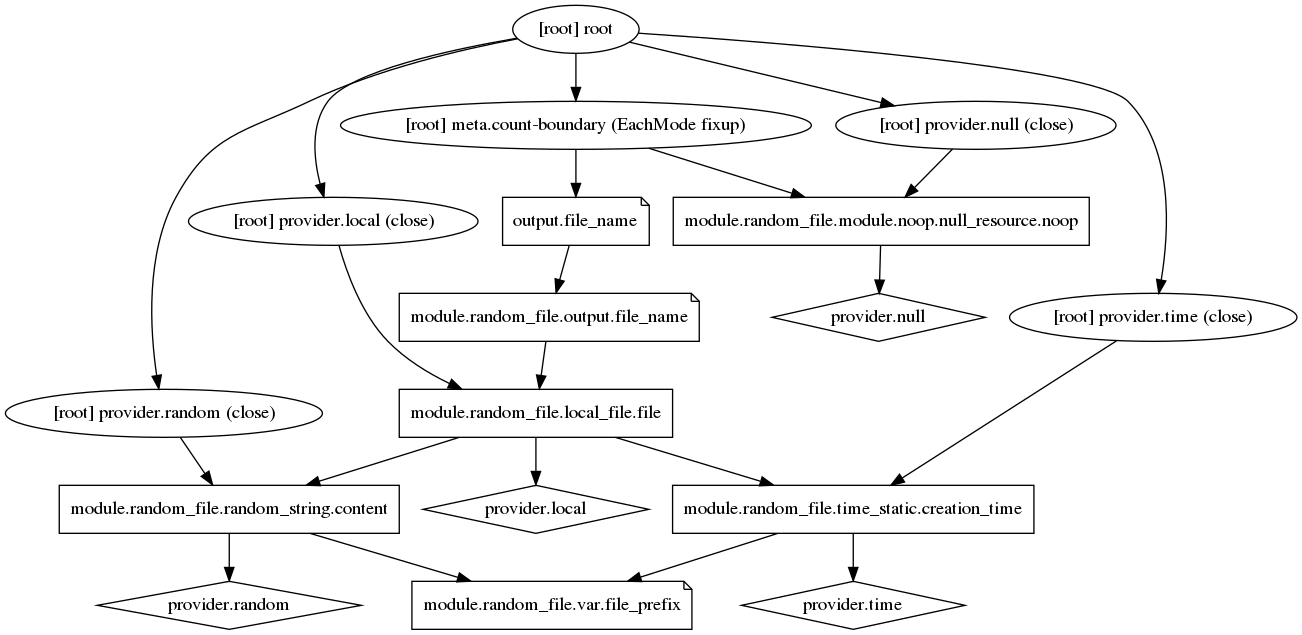
\includegraphics[keepaspectratio, height=7.5cm]{fig/hauptteil/terraform-graph.png}
  \caption{Beispiel Terraform Graph}
  \centering
\end{figure}

Das obenstehende Abbild zeigt einen \enquote{rohen} Graphen der direkt
von Terraform mithilfe des entsprechenden Befehls erstellt wurde.
Bereits dieses sehr kleine System wirkt schon leicht unübersichtlich,
mit wachsender Größe wird es zunehmend schwierig einen Überblick
über die einzelnen Komponenten und vor allem die Module eines Systems
zu behalten. In den unten stehenden Abbildungen, die von Terraform Graph
erstellt wurden, werden die Module farblich hervorgehoben.

\subsubsection{Konkreter Aufbau in Microsoft Azure}

\newpage
\begin{landscape}
\subsubsection{Konkreter Aufbau in Google Cloud Platform}
\begin{figure}[H]
  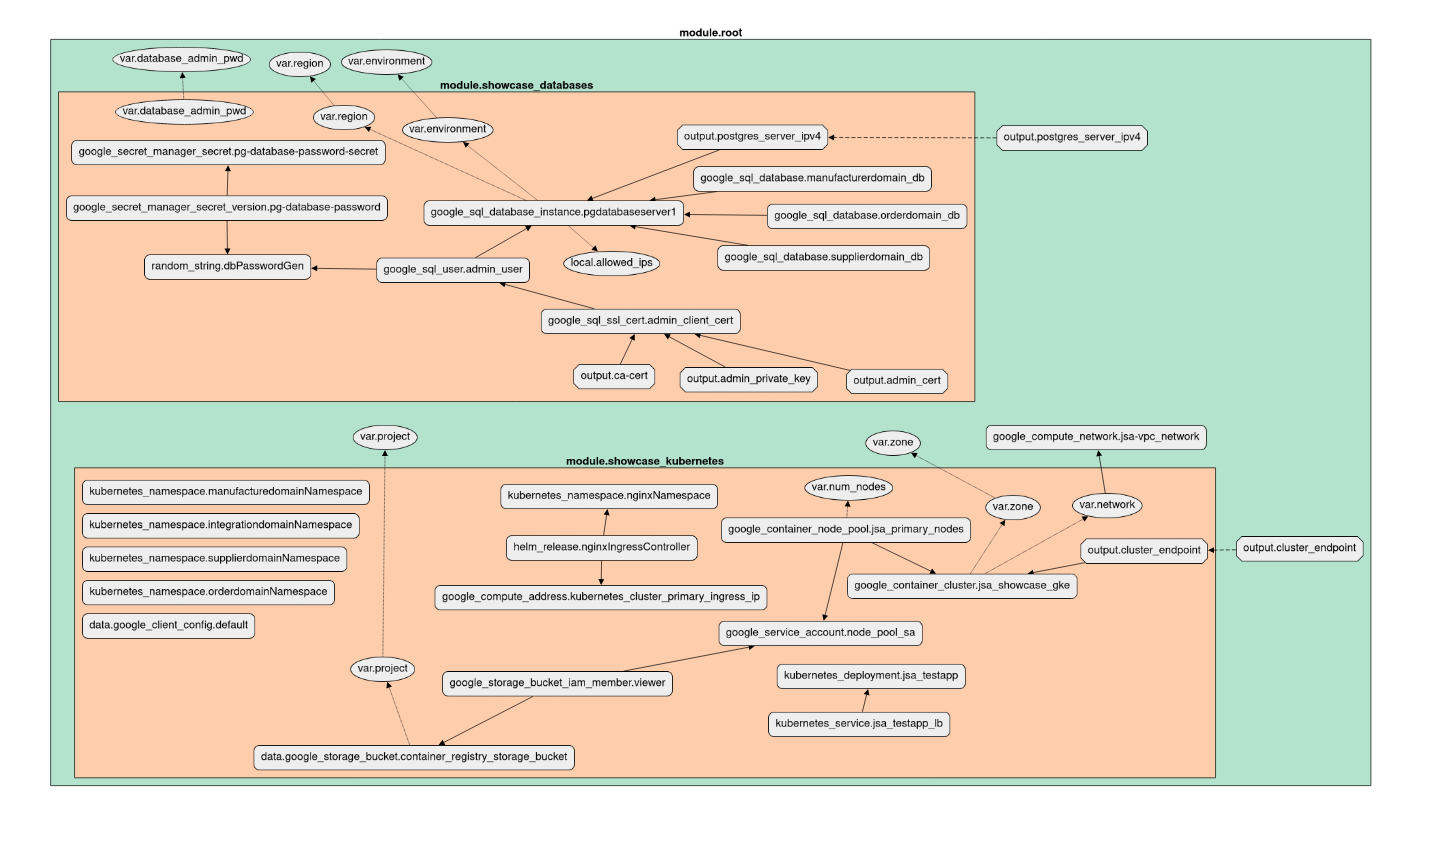
\includegraphics[keepaspectratio, height=13cm]{fig/hauptteil/gcp-terraform-graph-beautifier.png}
  \caption{Testsystem in Google Cloud Platform}
  \centering
\end{figure}
\end{landscape}

Eine Auffälligkeit in Google Cloud im Vergleich mit Microsoft Azure
ist der Secrets Storage der nur einmal projektweit existiert.
Zusätzlich war das anlegen der Container Registry nicht vollständig
ausgereift. Es existieren zwei Optionen: Die aktuelle Artifact
Registry deren Benutzung von Google empfohlen wird und die legacy
Container Registry. Die Artifact Registry war zum aktuellen Zeitpunkt
jedoch noch nicht vollständig im Terraform Provider implementiert,
es existierte keine Möglichkeit eine existierende Artifact Registry
als Data Source zu erfassen. Die Container Registry war daher die
einzige Option einen Speicherort für das Image im Vorfeld anzulegen
und in Terraform als Data Source einzubinden.\\
Weiterhin war es notwendig einen Serviceaccount anzulegen um das
Image aus der Registry zu laden und in den Nodes des Kubernetes
Clusters zu installieren.\\
Die weiteren Ressourcen konnten ohne weiteren Aufwand in einer
einfachen Weise implementiert und verwendet werden.

\subsection{Durchzuführende Messungen und Analysen}

\subsubsection{Functional completeness}

Eine essentielle Vorraussetzung für den Einsatz von Terraform ist die
Vollständigkeit der Funktionalitäten die für ein gegebenes
Infrastruktursystem erforderlich sind. Daher wird bei der
Implementierung des Testsystems als erstes analysiert ob alle
erforderlichen Ressourcen und Funktionalitäten in einer nutzbaren
Form vorhanden sind.

Betrachtet werden sollen die folgenden Ressourcen und
Funktionalitäten:

\begin{itemize}
  \item Anlegen virtueller Maschinen mit dem Betriebssystem Ubuntu 20.04.
  \item Anlegen eines PostgreSQL-Datenbankservers
  \item Anlegen mehrerer Datenbanken mit Charset UTF-8
  und Collation English\_United States.1252
  \item Anlegen eines Secret Storage
  \item Anlegen eines Kubernetes Cluster
  \item Erfassen einer Container Image Registry als Data Source
\end{itemize}

Zu beachten gilt dass das Referenzsystem in Microsoft Azure
implementiert ist weshalb alle Funktionalitäten dort entsprechend
garantiert sind.

\subsubsection{Time behaviour}

Eine weiterer kritischer Aspekt ist das das zeitliche Verhalten
von Terraform in Verbindung mit dem Terraform Provider und der
Cloud Plattform. Besonders in der Enwicklungsphase eines
Infrastruktursystems wird dieses oft ab- und wiederaufgebaut,
daher ist der zeitliche Aufwand der dafür benötigt wird von großer
Bedeutung.

Untersucht werden soll das zeitliche Verhalten der aufgelisteten
Systeme:

\begin{itemize}
  \item Das gesamte Versuchssystems
  \item Virtuelle Maschine mit dem Betriebssystem Ubuntu 20.04.
  \item PostgreSQL-Datenbankserver
  \item Kubernetes Cluster mit default Node Pool
\end{itemize}

Es werden sowohl die Dauer für den Auf- als auch Abbau gemessen.
Jeder Test wird drei mal wiederholt und der Mittelwert der
gemessenen Werte bewertet. Die Messungen werden nur durchgeführt
sofern die Plattform den Status der betroffenen Dienste als Normal/OK
führt. 

\subsubsection{Recoverability}

Für diesen Test wird zunächst der Aufbau des Systems angestoßen
durch das gewohnte \textit{terraform apply} angestoßen. Nach 
Ablauf von ca. der Hälfte der zum vollständigen Aufbau benötigten
Zeit wird die Internetverbindung im Betriebssystem manuell
unterbrochen.\\
Im Anschluss an diese Unterbrechung wird \textit{terraform apply}
erneut ausgeführt und überprüft ob die Ressourcen anschließend
zur Verfügung stehen. Sollte dies fehlschlagen wird der aufgetretene
Fehler dokumentiert.

Folgende Szenarien werden untersucht:

\begin{itemize}
  \item Virtuelle Maschine.
  \item PostgreSQL-Datenbankserver
  \item Datenbank unter Standardeinstellungen
  \item Kubernetes Cluster mit default Node Pool
\end{itemize}

\subsubsection{Modifiability}

Hier wird untersucht wie unterschiedliche Ressourcen auf eine
Modifikation reagieren. Mithilfe der jeweiligen Browserbasierten
GUI der Cloud Plattformen wird der Effekt beobachtet und dokumentiert.

Folgende Szenarien werden untersucht:

\begin{itemize}
  \item Änderung des Betriebssystems einer Virtuellen Maschine
  \item Vergrößerung der Festplatte einer Virtuellen Maschine
  \item Wechsel des Netzwerks
  einer Virtuellen Maschine
  \item Vergrößerung der Festplattengröße eines Datenbankservers
  \item Änderung des Charset einer Datenbank in einem PostgreSQL-Server
  \item Vergrößerung eines Node Pools von 2 auf 3 Nodes
\end{itemize}

\chapter{Ergebnisse und Bewertung}
\label{sec:ergeb}

\section{Evaluierung der Functional completeness}

\begin{table}[H]
  \centering
  \begin{tabular}{|p{0.22\linewidth}|p{0.35\linewidth}|p{0.35\linewidth}|}
    \hline
    & Google Cloud Platform & Microsoft Azure\\
    \hline
    VM Ubuntu 20.04 & 
    Funktionalität wird durch Ressource 
    google\_compute\_instance erfüllt. & 
    Funktionalität wird
    durch Ressource  azurerm\_virtual\_machine erfüllt.\\
    \hline
    PostgreSQL Datenbankserver & 
    Funktionalität wird durch Ressource google\_sql\_database\_instance
    erfüllt. &
    Funktionalität wird durch Ressource
    azurerm\_postgresql\_server erfüllt. \\
    \hline
    Anlegen von Datenbanken mit Charset UTF-8 und Collation
    English\_United States.1252 
    & Funktionalität wird durch Ressource google\_sql\_database teilweise
    erfüllt. Collation kann bei Erstellung nicht wie erwünscht
    definiert werden. Default ist en\_US.UTF8. &
    Funktionalität wird durch Ressource 
    azurerm\_postgresql\_database erfüllt. Charset und Collation werden
    bei  Erstellung definiert\\
    \hline
    Secret Storage & Funktionalität wird durch Ressource
    google\_secret\_manager\_secret erfüllt.
    Es existiert ein Secret Storage je Google Project. & 
    Funktionalität wird durch Ressource azurerm\_key\_vault\_secret
    erfüllt. Mehrere secret storages in Resource Group möglich.\\
    \hline
    Kubernetes Cluster &  Funktionalität wird durch Ressource
    google\_container\_cluster erfüllt.
    & Funktionalität wird durch Ressource
    azurerm\_kubernetes\_cluster erfüllt.\\
    \hline
    Einbindung von Container Registry als Data Source & 
    Funktionalität wird durch Data Source 
    google\_storage\_bucket erfüllt werden.
    & Funktionalität wird duch Data Source
    azurerm\_container\_registry erfüllt.\\
    \hline
  \end{tabular}
  \caption{Functional Completeness von GCP und Azure}
\end{table}

\newpage

\subsubsection{Bewertung}
Die grundlegenden Computing Ressourcen werden durch beide Terraform
Provider erwartungsgemäß bereitgestellt, im Detail liegen jedoch
einige Unterschiede vor.\\
Beim Anlegen der Datenbanken in GCP können die Funktionalitäten von
Azure nicht vollständig abgebildet werden, Anpassung an Charset und
Collation sind zum Zeitpunk des Erstellens nicht möglich.
Das Charset entspricht dem gewünschten Wert, die Collation jedoch
nicht.\\
Der Secret Storage wir auf GCP einmal für ein GCP Project angelegt,
Azure hingegen bietet die Möglichkeit mehrere Key Vaults innerhalb
einer Resource Group anzulegen. Die Speicherung des tatsächlichen Secret
in der Ressource google\_secret\_manager\_seceret\_version anstelle
des zuvor anzulegenden google\_secret\_manager\_seceret fällt
etwas unintuitiv aus\\
Die Container Registry wird in Google Cloud in Form eines normalen
Googe Storage Buckets angelegt. Die bevorzugte Methode zur Speicherung
eines Container Image in GCP stellt die Artifact Registry dar,
diese ist jedoch zum aktuellen Zeitpunkt noch nicht vollständig im
Terraform Provider implementiert. Es ist möglich eine Artifact
Registry als Terraform Ressource zu erstellen, die Einbindung einer
bereits bestehenden Artifact Registry als Data Source ist jedoch
noch nicht möglich. Der Aufwand beim Erstellen der Container Registry
über den Storage Bucket fällt höher aus als in Azure, hier wird beim
Anlegen der Container Registry die Storage-Infrastruktur automatisch
erstellt und gemanaged.

\section{Time behaviour Tests}

\begin{table}[H]
  \centering
  \begin{tabular}{|p{0.22\linewidth}|p{0.35\linewidth}|p{0.35\linewidth}|}
    \hline
    & Google Cloud Platform & Microsoft Azure\\
    \hline
    Aufbau/Abbau Testsystem & 
    Aufbau 1: 15m48s Abbau 1: 7m54s
    Aufbau 2: 17:37 Abbau 2: 8m11s
    Aufbau 3: 15m12s Abbau 3: 6m52 &
    Aufbau 1: 7m7s Abbau 1: 6m5s
    Aufbau 2: 7m59s Abbau 2: 7m44s
    Aufbau 3: 6m54s Abbau 3: 6m6s \\
    \hline
    Aufbau/Abbau VM &
    Aufbau 1: 0m30s Abbau 1: 1m3s
    Aufbau 2: 0m23s Abbau 2: 1m4s
    Aufbau 3: 0m25s Abbau 3: 1m4s &
    Aufbau 1: 1m12s Abbau 1: 1m36s
    Aufbau 2: 1m11s Abbau 2: 1m37s
    Aufbau 3: 1m11s Abbau 3: 1m40s \\
    \hline
    Aufbau/Abbau PostgreSQL-Datenbankserver &
    Aufbau 1: 3m49s Abbau 1: 1m3s
    Aufbau 2: 3m58s Abbau 2: 0m52s
    Aufbau 3: 3m57s Abbau 3: 0m52s &
    Aufbau 1: 2m28s Abbau 1: 0m42s
    Aufbau 2: 2m32s Abbau 2: 0m43s
    Aufbau 3: 2m28s Abbau 3: 0m40s \\
    \hline
    Aufbau/Abbau Kubernetes-Cluster mit default Node Pool &
    Aufbau 1: 3m59s Abbau 1: 2m52s
    Aufbau 2: 3m39s Abbau 2: 3m3s
    Aufbau 3: 3m31s Abbau 3: 2m53s &
    Aufbau 1: 4m36s Abbau 1: 5m33s
    Aufbau 2: 6m05s Abbau 2: 5m32s
    Aufbau 3: 5m13s Abbau 3: 5m29s \\
    \hline
    Terraform plan für Testsystem &
    Plan 1: 1.2s
    Plan 2: 1.2s
    Plan 3: 1.6s &
    Plan 1: 14.6s
    Plan 2: 15.2s
    Plan 3: 14.9s \\
    \hline
    Terraform plan für Datenbankserver &
    Plan 1: 0.9s
    Plan 2: 1.0s
    Plan 3: 1.0s &
    Plan 1: 22.2s
    Plan 2: 23.2s
    Plan 3: 23.3s \\
    \hline
    Terraform plan für Kubernetes-Cluster mit default Node Pool &
    Plan 1: 0.8s
    Plan 2: 0.9s
    Plan 3: 0.9s &
    Plan 1: 13.5s
    Plan 2: 13.3s
    Plan 3: 12.3s \\
    \hline
  \end{tabular}
  \caption{Time behaviour von GCP und Azure in verschiedenen Szenarien}
\end{table}

\subsubsection{Bewertung}

\section{Recoverability Tests}

\begin{table}[H]
  \centering
  \begin{tabular}{|p{0.22\linewidth}|p{0.35\linewidth}|p{0.35\linewidth}|}
    \hline
    & Google Cloud Platform & Microsoft Azure\\
    \hline
    Längere Unterbrechung des Internets, State in Remote Backend 
    &State korrumpiert, erneutes terraform apply führt zu Fehler, manuelles Entfernen der Ressource notwendig.
    &State korrumpiert, erneutes terraform apply führt zu Fehler, zusätzlich zur VM-Ressource muss die Festplatte
    ebenfalls separat manuell gelöscht werden.\\
    \hline
    Temporäre Unterbrechung des Internets, lokaler State
    &Terraform state wird auch lokal korrumpiert, manuelles löschen der
    VM-Ressource notwendig.
    &\\
    \hline
    \enquote{Soft Cancel} von Terraform Apply &
    State korrumpiert&
    Shutdown sofort, State korrumpiert\\
    \hline
    \enquote{Hard Cancel} von Terraform Apply &
    State korrumpiert&
    Nicht durchgeführt\\
    \hline
  \end{tabular}
  \caption{Recoverability von GCP und Azure in Bezug auf individuelle Ressourcen}
\end{table}

\subsubsection{Bewertung}

\section{Modifiability Tests}

\begin{table}[H]
  \centering
  \begin{tabular}{|p{0.22\linewidth}|p{0.35\linewidth}|p{0.35\linewidth}|}
    \hline
    & Google Cloud Platform & Microsoft Azure\\
    \hline
    Änderung des Betriebssystems einer Virtuellen Maschine &
    Ressource wird zerstört und neu erstellt. &
    Ressource wird zerstört und neu erstellt.\\
    \hline
    Vergrößerung der Festplatte einer Virtuellen Maschine &
    Ressource wird zerstört und neu erstellt.&
    Führt zu Error.\\
    \hline
    Veränderung des Machine-Type einer Virtuellen Maschine &
    Ressource wird modifiziert. &
    Ressource wird modifiziert.\\
    \hline
    Vergrößerung des default Node Pools von 1 auf 2 Nodes &
    Ressource wird zerstört und neu erstellt. &
    Ressource wird modifiziert. \\
    \hline
  \end{tabular}
  \caption{Modifiability von GCP und Azure in Bezug auf individuelle Ressourcen}
\end{table}

\subsubsection{Bewertung}

\end{spacing}